\documentclass[a4paper,11pt,twoside]{report}


% -------------- Kodowanie znaków, język polski -------------

\usepackage[utf8]{inputenc}
\usepackage[MeX]{polski}
%\usepackage[T1]{fontenc}
\usepackage[english, polish]{babel}


% ----------------- Przydatne pakiety ----------------------
\usepackage{amsfonts}
\usepackage{mathrsfs} 
\usepackage{amsmath,amsthm,latexsym,xpatch}
\usepackage[dvips]{graphicx,color}
\usepackage{enumerate}
\usepackage{enumitem}
\usepackage{verbatim}
\usepackage{array}
\usepackage{pstricks}
\usepackage{textcomp}


% ---------------- Marginesy, akapity, interlinia ------------------

\usepackage[inner=20mm, outer=20mm, bindingoffset=10mm, top=25mm, bottom=25mm]{geometry}


\linespread{1.5}
%\allowdisplaybreaks
\usepackage{indentfirst} % opcjonalnie; pierwszy akapit z wcięciem
\setlength{\parindent}{5mm}

\hyphenation{Syl-ves-tra}
\hyphenation{Syl-ves-ter-a}

%--------------------------- ŻYWA PAGINA ------------------------

\usepackage{fancyhdr}
\pagestyle{fancy}
\fancyhf{}
% numery stron: lewa do lewego, prawa do prawego 
\fancyfoot[LE,RO]{\thepage} 
% prawa pagina: zawartość \rightmark do lewego, wewnętrznego (marginesu) 
\fancyhead[LO]{\sc \nouppercase{\rightmark}}
% lewa pagina: zawartość \leftmark do prawego, wewnętrznego (marginesu) 
\fancyhead[RE]{\sc \leftmark}

\renewcommand{\chaptermark}[1]{
\markboth{\thechapter.\ #1}{}}

% kreski oddzielające paginy (górną i dolną):
\renewcommand{\headrulewidth}{0 pt} % 0 - nie ma, 0.5 - jest linia


\fancypagestyle{plain}{% to definiuje wygląd pierwszej strony nowego rozdziału - obecnie tylko numeracja
  \fancyhf{}%
  \fancyfoot[LE,RO]{\thepage}%
  
  \renewcommand{\headrulewidth}{0pt}% Line at the header invisible
  \renewcommand{\footrulewidth}{0.0pt}
}



% ---------------- Nagłówki rozdziałów ---------------------

\usepackage{titlesec}
\titleformat{\chapter}%[display]
  {\normalfont\Large \bfseries}
  {\thechapter.}{1ex}{\Large}

\titleformat{\section}
  {\normalfont\large\bfseries}
  {\thesection.}{1ex}{}
\titlespacing{\section}{0pt}{30pt}{20pt} 
%\titlespacing{\co}{akapit}{ile przed}{ile po} 
    
\titleformat{\subsection}
  {\normalfont \bfseries}
  {\thesubsection.}{1ex}{}


% ----------------------- Spis treści ---------------------------
\def\cleardoublepage{\clearpage\if@twoside
\ifodd\c@page\else\hbox{}\thispagestyle{empty}\newpage
\if@twocolumn\hbox{}\newpage\fi\fi\fi}


% kropki dla chapterów
\usepackage{etoolbox}
\makeatletter
\patchcmd{\l@chapter}
  {\hfil}
  {\leaders\hbox{\normalfont$\m@th\mkern \@dotsep mu\hbox{.}\mkern \@dotsep mu$}\hfill}
  {}{}
\makeatother

\usepackage{titletoc}
\makeatletter
\titlecontents{chapter}% <section-type>
  [0pt]% <left>
  {}% <above-code>
  {\bfseries \thecontentslabel.\quad}% <numbered-entry-format>
  {\bfseries}% <numberless-entry-format>
  {\bfseries\leaders\hbox{\normalfont$\m@th\mkern \@dotsep mu\hbox{.}\mkern \@dotsep mu$}\hfill\contentspage}% <filler-page-format>

\titlecontents{section}
  [1em]
  {}
  {\thecontentslabel.\quad}
  {}
  {\leaders\hbox{\normalfont$\m@th\mkern \@dotsep mu\hbox{.}\mkern \@dotsep mu$}\hfill\contentspage}

\titlecontents{subsection}
  [2em]
  {}
  {\thecontentslabel.\quad}
  {}
  {\leaders\hbox{\normalfont$\m@th\mkern \@dotsep mu\hbox{.}\mkern \@dotsep mu$}\hfill\contentspage}
\makeatother



% ---------------------- Spisy tabel i obrazków ----------------------

\renewcommand*{\thetable}{\arabic{chapter}.\arabic{table}}
\renewcommand*{\thefigure}{\arabic{chapter}.\arabic{figure}}
%\let\c@table\c@figure % jeśli włączone, numeruje tabele i obrazki razem


% --------------------- Definicje, twierdzenia etc. ---------------


\makeatletter
\newtheoremstyle{definition}%    % Name
{3ex}%                          % Space above
{3ex}%                          % Space below
{\upshape}%                      % Body font
{}%                              % Indent amount
{\bfseries}%                     % Theorem head font
{.}%                             % Punctuation after theorem head
{.5em}%                            % Space after theorem head, ' ', or \newline
{\thmname{#1}\thmnumber{ #2}\thmnote{ (#3)}}%  % Theorem head spec (can be left empty, meaning `normal')
\makeatother

% ----------------------------- POLSKI --------------------------------
\theoremstyle{definition}
\newtheorem{theorem}{Twierdzenie}[chapter]
\newtheorem{lemma}[theorem]{Lemat}
\newtheorem{example}[theorem]{Przykład}
\newtheorem{proposition}[theorem]{Stwierdzenie}
\newtheorem{corollary}[theorem]{Wniosek}
\newtheorem{definition}[theorem]{Definicja}
\newtheorem{remark}[theorem]{Uwaga}
\newtheorem{pseudokod}{Pseudokod}[subsection]

% If in English, comment this and uncomment below:

% ----------------------------- ENGLISH -----------------------------
%\theoremstyle{definition}
%\newtheorem{theorem}{Theorem}[chapter]
%\newtheorem{lemma}[theorem]{Lemma}
%\newtheorem{example}[theorem]{Example}
%\newtheorem{proposition}[theorem]{Proposition}
%\newtheorem{corollary}[theorem]{Corollary}
%\newtheorem{definition}[theorem]{Definition}
%\newtheorem{remark}[theorem]{Remark}



% ----------------------------- Dowód -----------------------------

\makeatletter
\renewenvironment{proof}[1][\proofname]
{\par
  \vspace{-12pt}% remove the space after the theorem
  \pushQED{\qed}%
  \normalfont
  \topsep0pt \partopsep0pt % no space before
  \trivlist
  \item[\hskip\labelsep
        \sc
    #1\@addpunct{:}]\ignorespaces
}
{%
  \popQED\endtrivlist\@endpefalse
  \addvspace{20pt} % some space after
}

\renewcommand{\qedhere}{\hfill \qedsymbol}
\makeatother





% -------------------------- POCZĄTEK --------------------------


% --------------------- Ustawienia użytkownika ------------------

\newcommand{\tytul}{Opracowanie modułu automatycznego parkowania samochodu}
\renewcommand{\title}{Design of automatic parking system for vehicle}
\renewcommand{\author}{Wojciech Kowalik}
\newcommand{\album}{254199}
\newcommand{\type}{magisters} % magisters, licencjac (Master or Engineer in English)
\newcommand{\supervisor}{prof. dr hab. inż. Krzysztof Marciniak}



\begin{document}
\sloppy

% \selectlanguage{english} % uncomment this for English 

% ----------------------- Abstrakty -----------------------------

%\selectlanguage{polish}
\begin{abstract}

\begin{center}
\tytul
\end{center}

Niniejsza praca dyplomowa opisuje proces powstawania aplikacji umożliwiającej planowanie ruchu pojazdu wyposażonego w moduł automatycznego parkowania. Aplikacja składa się z kilku modułów, takich jak: edytor map, edytor pojazdów, planer ruchu czy moduł wizualizacji. Ponadto możliwa jest zmiana wielu ustawień systemu takich jak wygląd rysowanych obiektów na mapie oraz jego język. Zgodnie z określonymi na wstępie wymaganiami aplikacja działa poprawnie na systemach operacyjnych z rodziny Windows począwszy od systemu Windows 7.

W pierwszym rozdziale przedstawione zostały cele pracy oraz dostępne publikacje, które zostały wykorzystane w trakcie pisania pracy. Drugi rozdział zawiera szczegółowe informacje na temat wymagań funkcjonalnych każdego z modułów, w które została wyposażona aplikacja oraz wymagania niefunkcjonalne dotyczące całego systemu. Najważniejszą funkcjonalnością edytora map i pojazdów jest możliwość utworzenia nowej mapy lub pojazdu oraz zapisania ich do pliku. Planer ruchu umożliwia wyznaczenie trajektorii po której będzie poruszał się pojazd z uwzględnieniem różnych parametrów, zadanych przez użytkownika. Moduł wizualizacji pozwala na wczytanie gotowej symulacji a następnie wizualizuje przejazd pojazdu z położenia początkowego do położenia końcowego zarówno w trybie 2D jak i 3D. Ostatni z modułów pozwala na zmianę ustawień aplikacji.

W kolejnym rozdziale zostały przedstawione technologie, które zostały wykorzystane przy implementacji. Cała aplikacja została napisana w języku C++, a jej graficzny interfejs użytkownika powstał przy użyciu zestawu bibliotek Qt. Ponadto wykorzystane zostały takie biblioteki jak Boost, NanoVG, czy OpenGL, między innymi do serializacji obiektów oraz przygotowania wizualizacji 3D.

Rozdziały czwarty i piąty szczegółowo opisują zasadę działania zaprojektowanych algorytmów planowania ruchu oraz automatycznego parkowania. Ponadto rozdziały te zawierają również testy zaprojektowanych algorytmów oraz przedstawiają w jakim kierunku powinny zmierzać dalsze prace nad algorytmami.

W szóstym rozdziale została przedstawiona dość szczegółowa instrukcja użytkownika, natomiast ostatni rozdział zawiera krótkie podsumowanie całej pracy.\\ 

\noindent \textbf{Słowa kluczowe:} planer, ruchu, trajektorii, pojazdu, autopilot, asystent, moduł, automatycznego, parkowania, asystent, graf, Voronoi, widoczności
\end{abstract}

\null\thispagestyle{empty}\newpage

{\selectlanguage{english}
\begin{abstract}

\begin{center}
\title
\end{center}

This thesis describes the process of creating application that allows to path planning for vehicle equipped with automatic parking system.  The application has been divided into four  basics modules: map editor, vehicle editor, path planner, visualisation. In addition, it is possible to change many system settings such as the appearance of the elements drawing on map or the language of the application. The program works properly on Windows operating systems family, starting from Windows 7.

The first chapter presents the objectives of this thesis and the available publications which were used during the writing of this diploma thesis. The second chapter describes in detail all functional requirements for each module and nonfunctional requirements for the whole system. The main functionality of the map and vehicle editor is to enable the user to create new map or vehicle and save them to the result file. Path planner allows to find the path for the vehicle taking into account various parameters set by user. Visualisation module allows to load simulation from the file and then play vehicle motion between start and end position. The last module contains application settings.

The next chapter presents technologies used for creating the application. The program was written in C++ programming language, but to create graphic user interface Qt library was used. Moreover the applications uses such libraries like Boost, NanoVG or Open GL for example to serialize objects or to render 3D visualisation.

The fourth and fifth chapters describes in detail path planning and parking algorithms. These chapters contains also tests of the designed algorithms and present their advantages and disadvantages.

The sixth chapter contains detialed user guide and the last chapter contains short resume of the whole diploma thesis.\\

\noindent \textbf{Keywords:} vehicle, path, trajectory, planner, autopilot, assistant, module, automatic, parking, graph, Voronoi, visibility
\end{abstract}}


\null\thispagestyle{empty}\newpage

\null \hfill Warszawa, dnia ..................\\

\par\vspace{5cm}

\begin{center}
Oświadczenie % Declaration - for English
\end{center}

\indent Oświadczam, że pracę \type ką pod
tytułem ,,\tytul '', której promotorem jest \supervisor \ wykonałem
samodzielnie, co poświadczam własnoręcznym podpisem.
\vspace{2cm}

% English:

%I hereby declare that the thesis entitled ,,\title '', submitted for the \type ~degree, supervised  by \supervisor , is entirely my original work apart from the recognized reference.
%\vspace{2cm}

\begin{flushright}
  \begin{minipage}{50mm}
    \begin{center}
      ..............................................

    \end{center}
  \end{minipage}
\end{flushright}

\thispagestyle{empty}
\newpage

\null\thispagestyle{empty}\newpage
% ------------------- 4. Spis treści ---------------------
% \selectlanguage{english} - for English

\tableofcontents
\thispagestyle{empty}
\newpage
% -------------- 5. ZASADNICZA CZĘŚĆ PRACY --------------------
\null\thispagestyle{empty}\newpage
\setcounter{page}{11}
\pagestyle{fancy}


\chapter*{Wstęp} % Intruduction
\markboth{}{Wstęp}
\addcontentsline{toc}{chapter}{Wstęp}

Jednym z największych wyzwań jakie czekają na kursantów ubiegających się o wydanie dokumentu prawa jazdy jest nauka manewru parkowania równoległego. Problem  ten nie dotyczy tylko młodych kierowców. Niejednokrotnie osoby posiadające prawo jazdy od kilku lat mają problem aby poprawnie zaparkować samochód w dość wąskim miejscu, a wykonanie idealnego manewru parkowania równoległego w jednym lub maksymalnie dwóch ruchach jest prawdziwą sztuką. W dzisiejszych czasach z pomocą przychodzą zaawansowane systemy parkowania automatycznego, które są już na wyposażeniu wszystkich wiodących marek produkujących samochody osobowe. 

Zazwyczaj mamy do czynienia z półautomatycznym systemem wspomagającym parkowanie (asystentem), który sam znajduje  wystarczającą do zaparkowania ilość miejsca, a także pomaga wykonać samą czynność odpowiednio sterując kierownicą. Jedynym zadaniem kierowcy jest odpowiednie operowanie pedałami gazu i hamulca. Jest to absolutnie podstawowa wersja asystenta parkowania, którą oferują nawet najprostsze i najtańsze rozwiązania. 


W przypadku bardziej zaawansowanych systemów parkowanie jest wykonywane w pełni automatycznie, a niekiedy możliwe jest nawet opuszczenie pojazdu przez kierowcę. Rozwiązania najbardziej zaawansowane dostarczają możliwość automatycznego wjazdu lub wyjazdu pojazdu z garażu bez obecności kierowcy w samochodzie.

Jak w praktyce wygląda działanie asystenta parkowania? Po pierwsze kierowca musi wybrać interesujący go tryb parkowania (prostopadłe lub równoległe), gdyż system zazwyczaj nie jest w stanie samodzielnie tego określić. Następnie rozpoczyna się proces wyszukiwania wolnego miejsca w czasie którego trzeba w miarę wolno jechać do przodu (zwykle maksymalnie 20-30 km/h). Gdy stosowne miejsce zostanie odnalezione komputer prosi o zatrzymanie się i najczęściej o włączenie biegu wstecznego. Od tego momentu komputer przejmuje pełną lub część kontroli nad pojazdem, w zależności od zaawansowania systemu. Oczywiście kierowca w dowolnym momencie może przerwać działanie systemu i samodzielnie kontynuować wykonywanie manewru. Cały proces parkowania zajmuje od kilkunastu do kilkudziesięciu sekund.

Zupełnie inną kategorię systemów wspomagających kierowcę stanowią autopiloty. Obecnie najwięksi producenci aut na świecie testują swoje rozwiązania, a rezultaty tych testów są bardzo obiecujące. Dla przykładu w grudniu 2016 roku konwój ciężarówek z powodzeniem zakończył testowy przejazd po Europie. Ciężarówki takich firm jak DAF, Daimler, IVECO, MAN, Scania i Volvo wyruszyły z różnych miejsc w Europie, m.in. ze Szwecji, Belgii i Niemiec. Za cel obrały Rotterdam w Holandii. Ciężarówki jechały samodzielnie w kolumnach składających się z 2-3 pojazdów i zachowywały stałe tempo jazdy. Były połączone ze sobą za pomocą Wi-Fi. To ciężarówka z przodu ustalała trasę i prędkość, a pozostałe za nią podążały. Nad komputerem czuwał jednak człowiek, który siedział na miejscu kierowcy. Wszystkie ciężarówki szczęśliwie dojechały do Rotterdamu. 

Innym przykładem ukazującym potencjał jaki drzemie w samochodowych autopilotach jest sytuacja jaka miała miejsce również w grudniu 2016 roku w Holandii. Kierowca poruszający się pojazdem marki Tesla Model X uniknął kolizji na autostradzie dzięki wczesnej reakcji systemu autopilota, który wykonał hamowanie, podczas gdy dla kierowcy niebezpieczeństwo nie było jeszcze widoczne przez kolejny ułamek sekundy. Widać więc, że zaawansowane systemy, w które obecnie wyposażane są samochody nie tylko podnoszą komfort jazdy, ale niekiedy potrafią ratować również ludzkie życie.

Niniejsza praca magisterska miała na celu opracowanie systemu, który umożliwia bezkolizyjny przejazd pojazdu z wyznaczonego miejsca i orientacji do miejsca docelowego. Dodatkowo pojazd ten został wyposażony w system automatycznego parkowania. W przygotowanej aplikacji użytkownik otrzymuje do dyspozycji edytor pozwalający na tworzenie/edycję map po których ma poruszać się pojazd, edytor pojazdów, planer ruchu, który odpowiedzialny jest za wyznaczenie ścieżki, biorąc pod uwagę różne parametry wprowadzane przez użytkownika oraz moduł wizualizacji, który jest dostępny zarówno w trybie 2D jak i 3D. 

W celu stworzenia aplikacji wykorzystany został język programowania C++, natomiast interfejs użytkownika został wykonany z wykorzystaniem zestawu bibliotek Qt. Do stworzenia edytorów oraz wizualizacji 2D wykorzystano bibliotekę NanoVG. Wizualizacja 3D została przygotowana w całości w technologii OpenGL.

\chapter{Cel pracy i dostępne publikacje}

Tematem niniejszej pracy dyplomowej było opracowanie modułu automatycznego parkowania dla samochodu. Jednak dodatkowo opracowany został planer ruchu, aby poza parkowaniem możliwe było również poruszanie się pojazdu pomiędzy zadanymi położeniami. Podczas implementacji systemu wykorzystano umiejętności zdobyte na studiach drugiego stopnia, specjalność „Projektowanie systemów CAD/CAM”, jak również informacje zawarte w kilku publikacjach dostępnych w Internecie. Ich krótki przegląd przedstawiono poniżej. 

\section{Parking Path Programming Strategy for Automatic Parking System}

Autorami tej publikacji są Jian-Min Wang, Sen-Tung Wum Chao-Wei Ke oraz Bo-Kai Tzeng. W publikacji opisany został algorytm wyznaczania ścieżki umożliwiającej zaparkowanie pojazdu w miejscu przeznaczonym do parkowania równoległego. Rozwiązanie zaproponowane przez autorów opiera się na założeniu, że parkowanie będzie odbywać się w jednym manewrze. Takie założenie wymusza więc, ze miejsce parkingowe musi mieć odpowiednią długość. Sam manewr parkowania sprowadza się do ruchu pojazdu po dwóch okręgach, które z założenia mają mieć identyczne promienie. Na początku pojazd porusza się po pierwszym z okręgów, a następnie następuje zmiana okręgu w momencie gdy tylna oś pojazdu znajduje się na wysokości początku miejsca parkingowego. Rozwiązanie przedstawione w tej publikacji stało się podstawą algorytmu parkowania zaimplementowanego na potrzeby tej pracy.
 
\begin{figure}[h!]
\centering
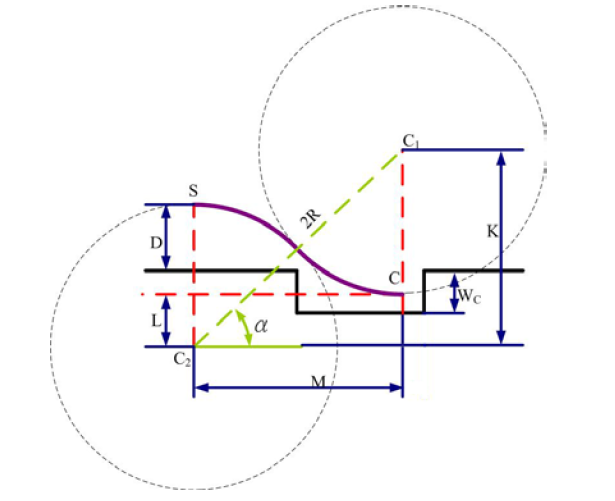
\includegraphics[scale=0.34]{parallelParking}
\caption[Manewr parkowania równoległego]{Manewr parkowania równoległego}
\end{figure} 
 
Autorzy publikacji poszli o krok dalej i poza opisem samego algorytmu parkowania zaprezentowali jego działanie w praktyce. W tym celu skonstruowali miniaturowy model pojazdu, który wyposażyli w odpowiednie czujniki. Parkowanie pojazdu przebiegło pomyślnie. Jednak ta część publikacji nie była już istotna z punktu widzenia niniejszej pracy.
 
\begin{figure}[h!]
\centering
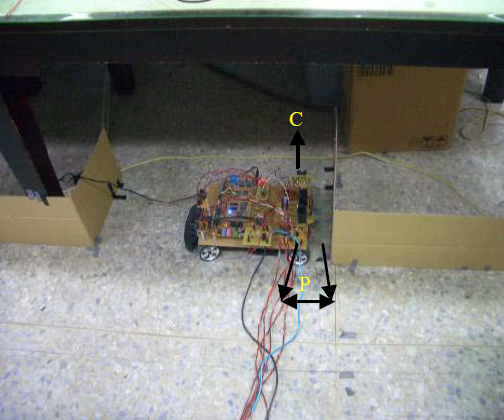
\includegraphics[scale=0.7]{miniVehicle}
\caption[Miniaturowy pojazd skonstruowany przez autorów publikacji]{Miniaturowy pojazd skonstruowany przez autorów publikacji}
\end{figure}

\section{Easy Path Planning and Robust Control for Automatic Parallel Parking}

Jest to kolejna publikacja, w której autorzy przedstawiają geometryczne metody wyznaczania ścieżki parkowania równoległego. Rozważania autorów rozpoczynają się od przeprowadzenia krótkiej analizy ruchu pojazdu oraz geometrycznego przedstawienia manewru skrętu. Przedstawione zostają okręgi, jakie pojazd zakreśla podczas wykonywania skrętu oraz matematyczne metody pozwalające na obliczenie parametrów każdego z tych okręgów.

\begin{figure}[h!]
\centering
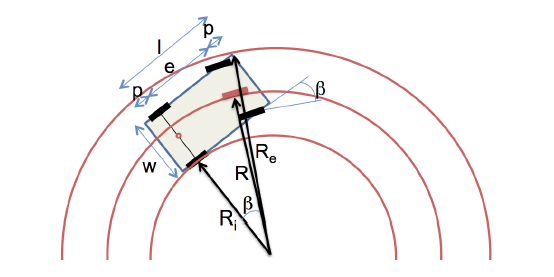
\includegraphics[scale=0.6]{easyPathPlanning1}
\caption[Okręgi zakreślane przez poruszający się pojazd]{Okręgi zakreślane przez poruszający się pojazd}
\end{figure}

W dalszej części dokumentu autorzy przechodzą do propozycji algorytmu parkowania równoległego. I tutaj podobnie jak w poprzedniej publikacji główna idea opiera się na poruszaniu się pojazdu po kolejnych łukach, gładko połączonych. W przeciwieństwie jednak do poprzedniej publikacji, autorzy nie ograniczają się wyłącznie do wyznaczenia trajektorii dla manewru parkowania które można wykonać w jednym manewrze, tylko analizują również przypadek, gdy miejsce parkingowe nie pozwala na taki manewr i pojazdu musi wykonać wiele ruchów do przodu i do tyłu, aż do momentu kiedy osiągnięta zostanie pozycja docelowa. 

\begin{figure}[h!]
\centering
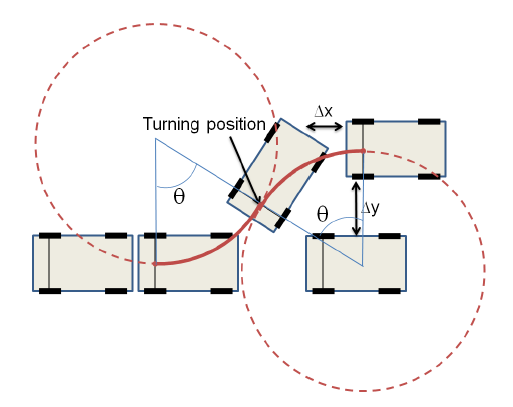
\includegraphics[scale=0.6]{easyPathPlanning2}
\caption[Pojazd poruszający się po kolejnych okręgach]{Pojazd poruszający się po kolejnych okręgach}
\end{figure}

Na koniec autorzy pokusili się jeszcze o przeprowadzenie analizy jak dużo miejsca potrzeba, aby pojazd o określonym maksymalnym kącie skrętu kół mógł zaparkować w jednym manewrze. Analiza ta została w mojej opinii przeprowadzona w bardzo dobry, a jednocześnie bardzo prosty sposób i jej wyniki również znajdują swoje zastosowanie w kolejnych rozdziałach niniejszej pracy.

\begin{figure}[h!]
\centering
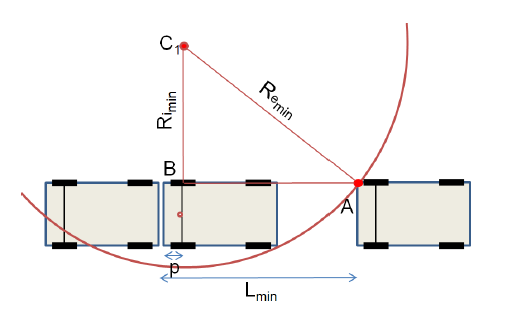
\includegraphics[scale=0.6]{easyPathPlanning3}
\caption[Minimalna długość miejsca parkingowego, aby możliwe było zaparkowanie w pojedynczym manewrze]{Minimalna długość miejsca parkingowego, aby możliwe było zaparkowanie w pojedynczym manewrze}
\end{figure}

\chapter{Analiza wymagań}

\section{Wymagania funkcjonalne}

Przygotowana aplikacja powinna zostać podzielona na 5 wymienionych poniżej modułów i dla każdego z nich spełniać określone wymagania funkcjonalne.

\subsection{Ekran startowy}

Ekran startowy to pierwszy widok ukazywany w aplikacji po jej uruchomieniu przez użytkownika. Powinien on zawierać informacje mówiące o tym czym jest ta aplikacja i w jakim celu powstała. Ponadto powinna być możliwość łatwego rozpoczęcia pracy z aplikacją bezpośrednio z ekranu startowego.

\subsection{Edytor map}

Głównym zadaniem edytora map jest umożliwienie użytkownikowi stworzenia nowej mapy o określonych wymiarach i zapisania jej do pliku. Ponadto możliwe powinno być również wczytanie uprzednio zapisanej mapy i dalsza jej edycja.

Po utworzeniu nowej mapy użytkownik powinien mieć możliwość dodawania następujących rodzajów obiektów:
\begin{itemize}
	\item budynków – podstawowym „budynkiem” powinna być prosta kostka sześcienna. Jest to wymaganie wstępne mające na celu ułatwienie procesu wytwarzania i testowania aplikacji. Po pomyślnym zaimplementowaniu obsługi zwykłego sześcianu jako budynku do aplikacji powinno zostać dodane kilka innych budynków posiadających własne siatki i tekstury,
	\item dekoracji – użytkownik powinien mieć możliwość umieszczania na mapie elementów dekoracyjnych takich jak drzewo, ławka itp. Na początek jednak podobnie jak w przypadku budynków wystarczy zaimplementować obsługę prostego sześcianu jako obiektu dekoracyjnego,
	\item miejsc parkingowych – powinno być możliwe dodawanie dwóch rodzajów miejsc parkingowych, przeznaczonych do parkowania równoległego oraz parkowania prostopadłego. Ponownie należy najpierw zaimplementować dwa typy będące prostymi powierzchniami, a następnie dodać modele o określonych wymiarach i z nałożonymi teksturami,
	\item pojazdów - użytkownik powinien mieć możliwość dodania do mapy pojazdów, które będą w tym wypadku przeszkodami podczas działania algorytmu planowania ruchu. Powinno dać się ustawić pojazd w dodanym wcześniej miejscu parkingowym.
\end{itemize}

Dla każdego z dodawanych obiektów użytkownik powinien mieć możliwość ustalenia jego nazwy oraz wykonywania na nim następujących operacji:
\begin{itemize}
	\item przesuwania (translacji),
	\item rotacji,
	\item skalowania.
\end{itemize}

Operacja skalowania nie jest jednak zalecana dla obiektów ze zdefiniowanymi siatkami i teksturami, czyli niebędących prostymi sześcianami, ponieważ może spowodować dziwne deformacje takiego obiektu, jeśli nie zostaną zachowane odpowiednie proporcje podczas operacji skalowania.

Dodatkowo podczas umieszczania obiektu na mapie oraz późniejszej jego edycji powinno się sprawdzać, czy obiekt ten nie koliduje z żadnym innym obiektem już umieszczonym na mapie oraz czy w całości mieści się w granicach mapy.

Kolejnym wymaganiem dla edytora map jest dodanie drzewa obiektów zawierającego wszystkie dodane do mapy obiekty. Przy tworzeniu drzewa powinien zostać uwzględniony podział na następujące gałęzie: budynki, dekoracje, miejsca parkingowe, pojazdy.

Ostatnim wymaganiem jest umożliwienie użytkownikowi zaznaczania dodanego już obiektu w celu jego ponownej edycji zarówno z poziomu drzewa obiektów jak i poprzez najechanie nad obiekt kursorem myszki i jego wybór. 

\subsection{Edytor pojazdów}

Edytor pojazdów jak sama nazwa wskazuje powinien umożliwiać użytkownikowi tworzenie oraz edycję uprzednio stworzonych pojazdów. Podobnie jak w edytorze map użytkownik powinien mieć możliwość utworzenia nowego pojazdu bądź wczytania lub zapisu. Podczas tworzenia nowego pojazdu użytkownik powinien mieć możliwość edycji następujących parametrów:
\begin{itemize}
	\item nazwy pojazdu,
	\item długości i szerokości pojazdu,
	\item rozstawu osi i kół w pojeździe,
	\item maksymalnego kąta skrętu przednich kół.
\end{itemize}

Ponadto edytor pojazdów powinien umożliwiać wczytanie następujących modeli 3D:
\begin{itemize}
	\item głównego modelu pojazdu,
	\item modelu lewego przedniego koła,
	\item modelu prawego przedniego koła,
	\item modelu lewego tylnego koła,
	\item modelu prawego tylnego koła.
\end{itemize}

Dodanie głównego modelu pojazdu jest wymagane i pojazd nie może być używany jeśli model ten nie zostanie dodany. Dodanie modeli poszczególnych kół nie jest wymagane, jednak zaleca się ich dodanie, ponieważ tylko wtedy możliwa będzie wizualizacja obrotu i skrętu kół. W przeciwnym wypadku model będzie traktowany jak jedna bryła i obrót, ani skręt kół nie będzie symulowany. Po dodaniu każdego z modeli kół powinno być możliwe jego poprawne ustawienie względem głównego modelu pojazdu poprzez translację, obroty i skalowanie.

\subsection{Planer ruchu}

Głównym zadaniem planera ruchu jest obliczanie trajektorii po jakiej ma poruszać się pojazd pomiędzy wskazanymi przez użytkownika położeniami lub miejscami parkingowymi. Planowanie ruchu powinno być dostępne dla następujących wariantów przejazdu:
\begin{itemize}
	\item położenie początkowe - położenie końcowe,
	\item miejsce parkingowe początkowe - położenie końcowe,
	\item położenie początkowe - miejsce parkingowe końcowe,
	\item miejsce parkingowe początkowe - miejsce parkingowe końcowe.
\end{itemize}

Użytkownik w dowolnym momencie pracy nad wyznaczeniem ścieżki powinien mieć możliwość resetu lub zapisania obecnych efektów pracy bądź wczytania uprzednio zapisanych danych z pliku.

Przed rozpoczęciem wyznaczania ścieżki, po której będzie poruszał się pojazd, użytkownik powinien skonfigurować następujące parametry:
\begin{itemize}
	\item mapa - możliwość importu z edytora map lub wczytania z pliku,
	\item pojazd - możliwość importu z edytora pojazdów lub wczytania z pliku,
	\item położenie/miejsce parkingowe początkowe,
	\item położenie/miejsce parkingowe końcowe.
\end{itemize}

Po ustawieniu powyższych parametrów powinna aktywować się opcja wyznaczania ścieżki, która do tej pory powinna pozostawać nieaktywna. Po jej wybraniu użytkownik powinien mieć możliwość skonfigurowania kolejnych parametrów, tym razem wykorzystywanych przez planer ruchu podczas konstrukcji trajektorii dla pojazdu. W skład tych parametrów wchodzą:
\begin{itemize}
	\item procentowa wartość informująca algorytm o tym o jaki procent szerokości pojazdu mają zostać powiększone przeszkody znajdujące się na mapie,
	\item rodzaj algorytmu planowania - do wyboru krzywa B-sklejana lub metoda wpisanych łuków,
	\item w przypadku wyboru algorytmu wykorzystującego wpisywane łuki, informacja czy pojazd może wykorzystywać dowolne czy tylko dopuszczalne dla swojej skrętności kół łuki,
	\item jakość sprawdzania i eliminacji kolizji pojazdu z innymi obiektami na mapie,
	\item liczbę dodawanych do grafu sztucznych wierzchołków w poziomie,
	\item liczbę dodawanych do grafu sztucznych wierzchołków w pionie.
\end{itemize}

Po zakończeniu wyznaczania ścieżki użytkownik powinien zostać poinformowany o powodzeniu lub niepowodzeniu tej operacji poprzez wyświetlenie stosownego komunikatu. Ponadto jeśli ścieżka została znaleziona użytkownik powinien mieć możliwość włączania i wyłączania wyświetlania następujących obiektów w celu zaprezentowania kolejnych kroków działania algorytmu planowania ruchu:
\begin{itemize}
	\item powiększonych przeszkód na mapie,
	\item grafu Voronoi,
	\item zmodyfikowanego grafu Voronoi,
	\item wyznaczonej łamanej będącej ścieżką pomiędzy zadanymi położeniami lub miejscami parkingowymi (o ile istnieje),
	\item wyznaczonych ścieżek parkowania (o ile takie istnieją),
	\item finalnie wyznaczonej trajektorii ruchu pojazdu (o ile istnieje).
\end{itemize}

\subsection{Wizualizacja}

Głównym zadaniem modułu wizualizacji jest wyświetlanie symulacji przejazdu samochodu zarówno w trybie 2D jak i 3D. Moduł wizualizacji powinien być wyposażony w listę symulacji, na której znajdują się uprzednio wczytane symulacje, które są gotowe do wyświetlenia użytkownikowi. Symulacje mogą być dodawane na listę na dwa sposoby:
\begin{itemize}
	\item import z modułu planera ruchu, pod warunkiem, że została tam przygotowana prawidłowa symulacja,
	\item wczytanie z uprzednio zapisanych plików. 
\end{itemize}

~\\Po zaznaczeniu symulacji na liście powinny aktywować się następujące opcje:
\begin{itemize}
	\item usunięcie symulacji z listy,
	\item wyświetlenie szczegółowych informacji o symulacji,
	\item możliwość odtworzenia/pauzowania lub zastopowania wybranej symulacji.
\end{itemize}

~\\Ponadto powinna być możliwość ustawienia czasu trwania symulacji przejazdu oraz wyświetlenie elementów wyznaczonej trajektorii w trybie 2D.

~\\Okno ze szczegółowymi informacjami na temat symulacji powinno zawierać następujące informacje:
\begin{itemize}
	\item długość znalezionej ścieżki,
	\item informację o jaki procent szerokości pojazdu powiększono obiekty na mapie,
	\item informację na temat wykorzystanego algorytmu planowania ruchu,
	\item informację, czy pojazd może wykonywać tylko dopuszczalne skręty,
	\item informację na temat dokładności sprawdzania kolizji wykorzystanej przy planowaniu ruchu,
	\item ilość dodanych sztucznych wierzchołków do grafu w pionie i w poziomie.
\end{itemize}

\newpage

\subsection{Ustawienia}

Podstawowym parametrem, którego zmianę powinien umożliwiać moduł ''Ustawienia'' jest język aplikacji. Domyślnie do wyboru powinien być język polski i angielski. Użytkownik może dodać dowolny język do aplikacji poprzez utworzenie dodatkowego pliku *.ini w katalogu, w którym znajduje się plik wykonywalny i nazywając go \textit{lang.kodKraju.ini}. Nowy język powinien być widoczny na liście języków do wyboru po restarcie aplikacji. Ponadto wybór języka powinien być zapamiętywany i po ponownym uruchomieniu aplikacji powinien być wybierany język poprzednio wybrany przez użytkownika.

Kolejnymi parametrami, których zmianę powinien umożliwiać moduł ''Ustawienia'' są parametry określające wygląd poszczególnych obiektów rysowanych w trybie widoku 3D. Powinno dać się zmodyfikować wygląd przynajmniej następujących elementów:
\begin{itemize}
	\item poszczególne elementy mapy: budynki, dekoracje, itp.,
	\item elementy wchodzące w skład generowanej trajektorii: linie, łuki, krzywe sklejane,
	\item wierzchołki i krawędzie wyświetlanych grafów.
\end{itemize}

\section{Wymagania niefunkcjonalne}

Poza wymienionymi powyżej wymaganiami funkcjonalnymi aplikacja powinna spełniać również pewne wymagania niefunkcjonalne. Najważniejszym z nich jest poprawne działanie aplikacji na systemach operacyjnych z rodziny Windows. Ponadto aplikacja powinna łatwo dać się tłumaczyć na inne języki oraz posiadać wbudowany język polski i angielski, a jej interfejs powinien być responsywny i prezentować się dobrze na monitorach o minimalnej rozdzielczości 1440×900 pikseli.

\chapter{Technologia}

W tym rozdziale zostaną przedstawione technologie, które wykorzystano w celu realizacji wymagań opisanych w poprzednim rozdziale.

Całość aplikacji została napisana w języku C++ z wykorzystaniem zestawu bibliotek ułatwiających tworzenie graficznego interfejsu użytkownika – Qt w wersji 5.8. Ponadto w celu implementacji zapisywania i wczytywania map, pojazdów oraz symulacji, a także do konstrukcji grafu Voronoi wykorzystano kolekcję bibliotek Boost w wersji 1.64. Edytory graficzne takie jak edytor map czy planer ruchu zostały zaimplementowane z wykorzystaniem biblioteki NanoVG, natomiast do przygotowania edytora pojazdów i wizualizacji 3D użyta została technologia OpenGL w połączeniu z kilkoma innymi bibliotekami, co zostanie opisane poniżej. 

\section{Qt 5.8}

Qt to zestaw przenośnych bibliotek i narzędzi programistycznych dedykowanych dla języków C++, QML i Java. Podstawowym składnikiem bibliotek wchodzących w skład Qt są klasy służące do budowy graficznego interfejsu użytkownika. Interfejs można budować pisząc kod lub przy pomocy edytora graficznego. Podczas stylizacji poszczególnych kontrolek możliwe jest użycie styli CSS. Poniżej zaprezentowano przykład stylizacji przycisku oraz zmiany jego wyglądu na akcje najechania myszką nad przycisk oraz jego wciśnięcia. W podobny sposób można zmieniać wygląd dowolnego elementu wchodzącego w skład interfejsu użytkownika.

\begin{pseudokod}
Przykład stylizacji przycisku w Qt
\begin{verbatim}
    QPushButton#idPrzycisku {
        background-color: #3b3e41;
        border: 1px solid #757575;
        font: bold 12px;
        color: white;
    }
    
    //stylizacja wyglądu po najechaniu myszką nad przycisk
    QPushButton#idPrzycisku:hover {
        background-color: #85b448;
    }
    
    //stylizacja wyglądu po naciśnięciu przycisku
    QPushButton#idPrzycisku:pressed {
        background-color: #d86a39;
    }
\end{verbatim}
\end{pseudokod}

\begin{figure}[h!]
\centering

\includegraphics[scale=1.0]{QPushButton}
\caption[Przykład stylizacji przycisku w Qt]{Przykład stylizacji przycisku w Qt}
\end{figure}

Począwszy od wersji 4.0 Qt zawiera również narzędzia służące do tworzenia programów konsolowych i serwerów. W opracowanym systemie Qt został wykorzystany wyłącznie do stworzenia graficznego interfejsu użytkownika.

\section{Boost 1.64}

Boost jest zbiorem bibliotek programistycznych rozszerzających możliwości języka C++. Dziedziny zastosowania Boost są bardzo szerokie. Pakiet dostarcza m.in. biblioteki ogólnego przeznaczenia (inteligentne wskaźniki, wyrażenia regularne), biblioteki stanowiące warstwę abstrakcji dla systemu operacyjnego (obsługa systemów plików czy wielowątkowości), jak i narzędzia przeznaczone głównie dla innych twórców bibliotek i zaawansowanych programistów języka C++ (np. biblioteka metaprogramowania MPL). Kilka bibliotek wchodzących w poczet Boost zostało włączonych do pierwszego raportu technicznego komitetu standaryzacyjnego C++, który jest zbiorem proponowanych rozszerzeń biblioteki standardowej języka C++. 

W przygotowanej aplikacji kolekcja bibliotek Boost została wykorzystana do implementacji zapisywania i wczytywania map, pojazdów oraz symulacji, a także do konstrukcji grafu Voronoi na podstawie przygotowanej przez użytkownika mapy.  Przykład wykorzystania biblioteki Boost do serializacji obiektu został przedstawiony poniżej.

\begin{pseudokod}
Przykład serializacji obiektu z wykorzystaniem biblioteki Boost
\begin{verbatim}
    // fragment serializujący dodany do klasy Model3D
    template<class Archive>
    void serialize(Archive & ar, const unsigned int version)
    {
        ar & position;
        ar & rotation;
        ar & scale;
    }
    ...
    // utworzenie strumienia w oparciu o podaną ścieżkę
    std::ofstream ofs("nazwaPliku");
    // utworzenie instancji obiektu
    const Model3D model;
    // serializacja obiektu 
    boost::archive::text_oarchive oa(ofs);
    oa << g;
\end{verbatim}
\end{pseudokod}

\section{NanoVG}

NanoVG jest kompaktową biblioteką wspierającą renderowanie grafiki wektorowej z antyaliasingiem dla OpenGL. Interfejs biblioteki jest bardzo zbliżony do interfejsu jaki dostarcza obiekt Canvas z HTML5 dzięki czemu osoby znające HTML5 mogą niemal natychmiast rozpocząć efektywną pracę z biblioteką NanoVG. Biblioteka ta powstała z myślą o dostarczeniu niewielkiego i prostego API, przy pomocy którego możliwe będzie tworzenie skalowalnych interfejsów użytkownika, wizualizacji czy wszelkiego rodzaju edytorów. Przykład użycia biblioteki przedstawiono poniżej.

\begin{pseudokod}
Przykład rysowania z wykorzystaniem biblioteki NanoVG
\begin{verbatim}
    nvgBeginPath(vg);
    nvgEllipse(vg, position.x, position.y, radius, radius);
    nvgFillColor(vg, color);
    nvgFill(vg);
\end{verbatim}
\end{pseudokod}

Potencjał biblioteki NanoVg ukazuje przykładowy interfejs użytkownika przygotowany przez jej autorów. Poniżej przedstawiono zrzut ekranu prezentujący ten interfejs.

\begin{figure}[h!]
\centering
\includegraphics[scale=0.8]{NanoVGInterface}
\caption[Przykładowy interfejs przygotowany z użyciem biblioteki NanoVG]{Przykładowy interfejs przygotowany z użyciem biblioteki NanoVG}
\end{figure}

\section{OpenGL}

OpenGL obok DirectX i Vulkan API jest podstawową niskopoziomową biblioteką graficzną 3D, obsługiwaną przez wszystkie liczące się systemy operacyjne oraz większość dostępnych na rynku procesorów graficznych. Niezależność od platformy sprzętowej oraz ogólnie dostępna specyfikacja czyni z OpenGL standard powszechnie wykorzystywany przez producentów oprogramowania użytkowego i gier. Zestaw funkcji OpenGL składa się z 250 podstawowych wywołań, umożliwiających budowanie złożonych trójwymiarowych scen z podstawowych figur geometrycznych.

Dzięki wykorzystaniu OpenGL w opracowanej aplikacji możliwe było stworzenie wydajnej wizualizacji 3D. Jako, że czysty OpenGL skupia się na dostarczaniu API służącego do komunikacji z procesorem karty graficznej i nie posiada takich narzędzi jak np. parsery plików z siatkami, to konieczne było użycie dodatkowych, dedykowanych bibliotek dla OpenGL. Najważniejsze z nich wymieniono poniżej:
\begin{itemize}
	\item GLEW - biblioteka pomagająca w odpytywaniu i ładowaniu rozszerzeń OpenGL. GLEW dostarcza efektywne mechanizmy do określania w czasie uruchamiania programu dostępnych rozszerzeń na danej platformie. Wszystkie rozszerzenia OpenGL są wylistowane w jednym pliku nagłówkowym, który z kolei jest maszynowo generowany na podstawie oficjalnej listy rozszerzeń.
	\item GLM - dostarcza zestaw obiektów i funkcji matematycznych zaprojektowanych pod kątem użycia ich w OpenGL oraz w konwencji nazewniczej języka GLSL.
	\item SOIL - biblioteka dostarczająca mechanizm umożliwiający wczytywanie obrazków oraz tekstur 3D do OpenGL. Biblioteka obsługuje wszystkie najpopularniejsze formaty.
	\item ASSIMP - biblioteka umożliwiająca łatwe załadowanie modeli 3D wraz z ich materiałami i innymi właściwościami do OpenGL. Biblioteka ta, podobnie jak biblioteka SOIL obsługuje wszystkie najpopularniejsze formaty modeli 3D. Ponadto, jeśli zostaną ustawione odpowiednie parametry, to biblioteka ASSIMP już na etapie wczytywania jest w stanie dokonać optymalizacji wczytywanych siatek 3D.
\end{itemize}

Użycie powyższych bibliotek w połączeniu z OpenGL jest w dzisiejszych czasach standardem.

\chapter{Analiza ruchu pojazdu}

Podczas analizy ruchu pojazdu w opracowanym systemie uwzględniona została tzw. geometria Ackermana (lub mechanizm kompensacji Ackermana), aby w możliwie realistyczny sposób opisać ruch prawdziwego pojazdu. Ponadto przyjęto założenie, że w każdym momencie ruchu pojazd porusza się z prędkością, która nie powoduje poślizgu bocznego. W poniższej analizie jako pozycję pojazdu przyjęto środek jego tylnej osi, natomiast w aplikacji ze względów technicznych jako środek pojazdu przyjmowany jest geometryczny środek otaczającego go prostokąta. Nie zmienia to jednak w żaden sposób opisywanych metod i specyfiki problemu.

\section{Geometria Ackermana}

Oczywistym jest fakt, iż podczas ruchu pojazdu w linii prostej oba przednie (skrętne) koła pozostają równoległe do siebie, a ich kąt skręcenia wynosi 0 stopni. Jednak w przypadku pokonywania nawet najmniejszego zakrętu, kąty skręcenia obu kół stają się różne. Za odpowiedni kąt skręcenia każdego z kół odpowiada mechanizm kompensacji Ackermana. Zastosowanie tego mechanizmu w pojazdach jest niezbędne, aby mogły one poruszać się po krzywiźnie bez poślizgu kół jezdnych, który mógłby spowodować utratę kontroli nad pojazdem, a w najlepszym wypadku przedwczesne zużycie się opon. Schemat działania mechanizmu kompensacji Ackermana został przedstawiony na rysunku 4.1.

\begin{figure}[h!]
\centering
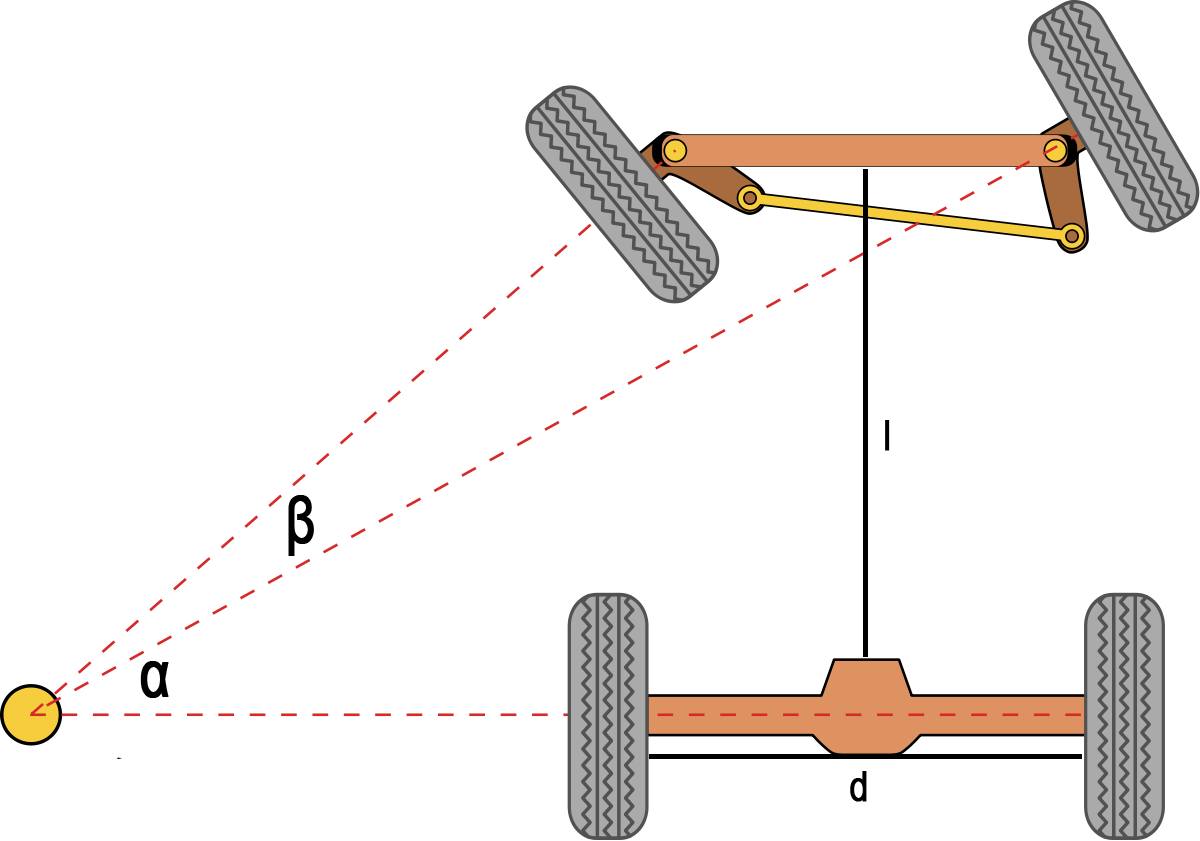
\includegraphics[scale=0.2]{ackermanGeometry}
\caption[Geometria Ackermana]{Geometria Ackermana}
\end{figure}

~\\Matematyczną zależność pomiędzy wartościami każdego z kątów określa następujące równanie, zwane też równaniem Ackermana:
$$
\ctg{\beta} - \ctg{\alpha} = \frac{d}{l},
$$
gdzie:
\begin{itemize}
	\item $\alpha, \beta$ - kąty skrętu odpowiednio zewnętrznego i wewnętrznego koła skrętnego,
	\item $l$ - rozstaw osi,
	\item $d$ - rozstaw kół.
\end{itemize}
\newpage

\section{Wyznaczanie minimalnego promienia skrętu}

Minimalny promień skrętu każdego pojazdu zależny jest od maksymalnego kąta skręcenia jego przednich kół, a precyzyjniej od maksymalnego kąta skręcenia koła znajdującego się po wewnętrznej stronie zakrętu (co wynika z geometrii Ackermana). Samo pojęcie minimalnego promienia skrętu również wymaga doprecyzowania, gdyż można rozważać wiele różnych promieni skrętu, w zależności od przyjętego punktu odniesienia na pojeździe. W poniższej analizie wyznaczone zostaną trzy promienie skrętu:
\begin{itemize}
	\item dla tylnego koła znajdującego się po wewnętrznej stronie zakrętu - $R_{min}$,
	\item dla przedniego koła znajdującego się po zewnętrznej stronie zakrętu - $R_{max}$,
	\item dla środka tylnej osi poruszającego się pojazdu - $R$.
\end{itemize}

Na poniższym rysunku zaznaczone zostały okręgi zakreślane przez skręcający pojazd oraz poszukiwane promienie.

\begin{figure}[h!]
\centering
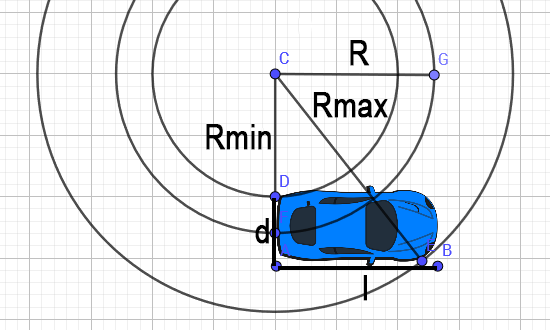
\includegraphics[scale=0.4]{vehicleTurningRadius}
\caption[Okręgi zakreślane przez skręcający pojazd i zaznaczone promienie]{Okręgi zakreślane przez skręcający pojazd i zaznaczone promienie}
\end{figure}

Do wykonania obliczeń zakładamy, że znamy rozstaw osi ($l$) oraz rozstaw kół pojazdu ($d$), a także kąt skręcenia wewnętrznego koła przedniego ($\beta$), który przy wyznaczaniu minimalnego promienia skrętu musi być równy maksymalnemu kątowi skrętu kół dla danego pojazdu (na ogół wartość ta waha się w granicach 36-42 stopnie). Zaznaczone na rysunku promienie obliczamy w następujący sposób:

\begin{itemize}
	\item $R_{min} = \frac{l}{\tg{\beta}}$
	\item $R_{max} = \frac{l}{\sin{(outsideAngle)}}, \quad outsideAngle = \arctan{\frac{l}{R_{min} + d}}$
	\item $R = R_{min} + \frac{d}{2}$
\end{itemize}

\section{Wyznaczanie okręgów skrętu}

Pojazd znajdujący się w określonym położeniu posiada zawsze dwa okręgi po których natychmiast może zacząć się poruszać przy zadanym kącie skrętu kół w jedną lub drugą stronę. W systemie przyjęto założenie, że koła są zawsze maksymalnie skręcone, tak aby pojazd jak najwięcej poruszał się po liniach prostych, a zakręty pokonywał jak najszybciej. Pojazd z zaznaczonymi okręgami skrętu został przedstawiony na poniższym rysunku.

\begin{figure}[h!]
\centering
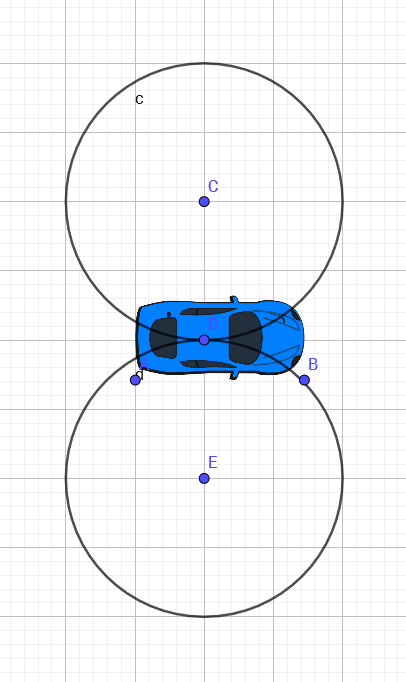
\includegraphics[scale=0.55]{vehicleWithTurningCircles}
\caption[Pojazd i jego okręgi skrętu]{Pojazd i jego okręgi skrętu}
\end{figure}

W poprzednim podrozdziale została opisana metoda wyznaczania różnych promieni skrętu. Do opisu pojedynczego okręgu skrętu oprócz jego promienia potrzebna jest informacja na temat położenia jego środka. Uzyskanie takiej informacji nie stanowi większego problemu i środki obu okręgów można obliczyć w następujący sposób:
$$
center = vehiclePosition \pm \Big(R_{min} + \frac{d}{2}\Big) \cdot dirTrack,
$$
gdzie: 
\begin{itemize}
	\item $vehiclePosition$ - akutalna pozycja pojazdu,
	\item $R_{min}$ - minimalny promień skrętu pojazdu,
	\item $d$ - rozstaw kół,
	\item $dirTrack$ - wektor określający kierunek tylnej osi pojazdu.
\end{itemize}

\chapter{Algorytmy planowania ruchu i parkowania}

Podczas implementacji aplikacji opracowano algorytm planowania ruchu pojazdu pomiędzy zadanymi położeniami oparty na krzywych B-sklejanych oraz na wpisywaniu łuków w łamaną złożoną z krawędzi grafu. Zaimplementowany został również algorytm parkowania równoległego i prostopadłego. Opracowane algorytmy zostały opisane w dalszej części tego rozdziału.

\section{Algorytm planowania ruchu}

Algorytmy planowania ruchu pojazdu można podzielić na dwa rodzaje - takie w których możliwe jest sprowadzenie pojazdu do punktu poprzez odpowiednie powiększenie przeszkód oraz takie w których tego zrobić nie można. Algorytmy pierwszego rodzaju można stosować przy założeniu, że pojazd, dla którego planowana jest trajektoria może obracać się w miejscu, wokół uprzednio zdefiniowanej osi obrotu. W takim wypadku przy obliczaniu trajektorii najczęściej wykorzystywane są tzw. grafy widoczności. Jeśli zaś sprowadzenie pojazdu do punktu nie jest możliwe to do wyznaczenia trajektorii można wykorzystać graf Voronoi.

Ponieważ w niniejszej pracy rozważany jest ruch pojazdu możliwie jak najbardziej zbliżony do ruchu prawdziwego samochodu, to algorytmy oparte o grafy widoczności zostaną pominięte i rozważane będą tylko algorytmy, w których niemożliwe jest zastąpienie pojazdu pojedynczym punktem.

\subsection{Idea algorytmu}

Podstawowymi parametrami wejściowymi dla algorytmu planowania ruchu pojazdu są następujące obiekty:
\begin{itemize}
	\item mapa
	\item pojazd - zawiera informację o maksymalnym skręcie kół, rozstawie osi oraz rozstawie kół,
	\item pozycja początkowa,
	\item pozycja końcowa.
\end{itemize}

Zdefiniowane powyżej parametry są niezbędne do rozpoczęcia planowania ruchu pojazdu. Sam proces wyznaczania trajektorii w najprostszej wersji można podzielić na następujące etapy:
\begin{itemize}
	\item jeśli położeniem początkowym lub końcowym jest miejsce parkingowe, to należy wyznaczyć trajektorię parkowania zgodnie z algorytmem, który zostanie opisany w następnym podrozdziale,
	\item utworzyć graf Voronoi, dla zadanej przez użytkownika mapy oraz dodać do niego wierzchołki reprezentujące położenie początkowe i końcowe oraz krawędzie do tych wierzchołków,
	\item wyznaczyć ścieżkę w grafie pomiędzy wierzchołkiem początkowym i końcowym, np. za pomocą algorytmu A*,
	\item na podstawie wyznaczonej łamanej, którą tworzą krawędzie wchodzące w skład ścieżki w grafie wyznaczyć trajektorię dopuszczalną dla pojazdu - przy pomocy krzywej sklejanej lub wpisując łuki pomiędzy kolejne odcinki łamanej.
\end{itemize}

Skuteczność opisanego powyżej algorytmu w praktyce była niewielka, dlatego na potrzeby tej pracy przebadano i opracowano następujące modyfikacje przedstawionego powyżej schematu:
\begin{itemize}
	\item powiększanie przeszkód,
	\item modyfikacja grafu Voronoi i ewentualne uzupełnienie go o dodatkowe wierzchołki i krawędzie,
	\item iteracyjne sprawdzanie i eliminacja kolizji.
\end{itemize}

W następnych podrozdziałach zostaną opisane wymienione powyżej modyfikacje, a także zostanie opisana metoda konstrukcji finalnej ścieżki oparta na krzywej sklejanej oraz wpisywaniu łuków pomiędzy odcinki łamanej.

\subsubsection{Powiększanie przeszkód}

Celem powiększania przeszkód na mapie jeszcze przed wyznaczeniem grafu Voronoi jest minimalizacja ryzyka kolizji pojazdu z danym obiektem, poprzez oddalenie krawędzi grafu od brzegów obiektu. Algorytm powiększania obiektów mapy jest bardzo prosty i sprowadza się do przesunięcia każdego wierzchołka wzdłuż normalnej do danej krawędzi przeszkody o odległość zdefiniowaną przez użytkownika (procentowa wartość szerokości pojazdu). Efektem zastosowania takiego algorytmu powiększania jest powstawanie przeszkód, które mają aż 8 wierzchołków ze standardowych przeszkód czworokątnych. Dzieje się tak, gdyż tak naprawdę każdy wierzchołek modyfikowanej przeszkody wejściowej jest przesuwany dwukrotnie, najpierw wzdłuż normalnej do jednej krawędzi, a następnie wzdłuż normalnej do krawędzi do niej prostopadłej. Przykład przeszkody przed powiększeniem i po powiększeniu zaprezentowano na obrazku poniżej.

\begin{figure}[h!]
\centering
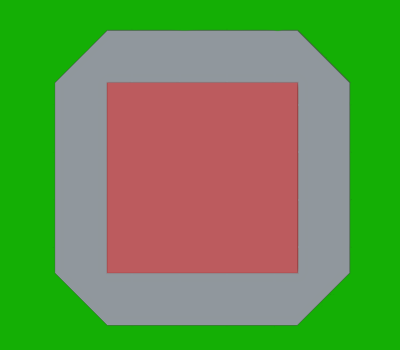
\includegraphics[scale=0.5]{expandObstacleExample}
\caption[Przykład powiększania przeszkody]{Przykład powiększania przeszkody}
\end{figure}

Dodatkowym efektem powiększenia przeszkód jest zupełnie inna postać wyznaczonego grafu Voronoi. Graf wyznaczony dla mapy ze standardowymi przeszkodami przed powiększeniem jest dużo prostszy i na pierwszy rzut oka ''czytelniejszy'', jednak bardziej wartościowy z punktu widzenia algorytmu planowania ruchu jest graf wyznaczony dla mapy z powiększonymi przeszkodami, ponieważ zawiera więcej wierzchołków i krawędzi, oraz minimalizuje ryzyko kolizji z przeszkodami poprzez zachowanie odpowiedniej odległości krawędzi od przeszkód. Porównanie obu grafów przedstawiają poniższe rysunki 5.2 oraz 5.3.

\begin{figure}[h!]
\centering
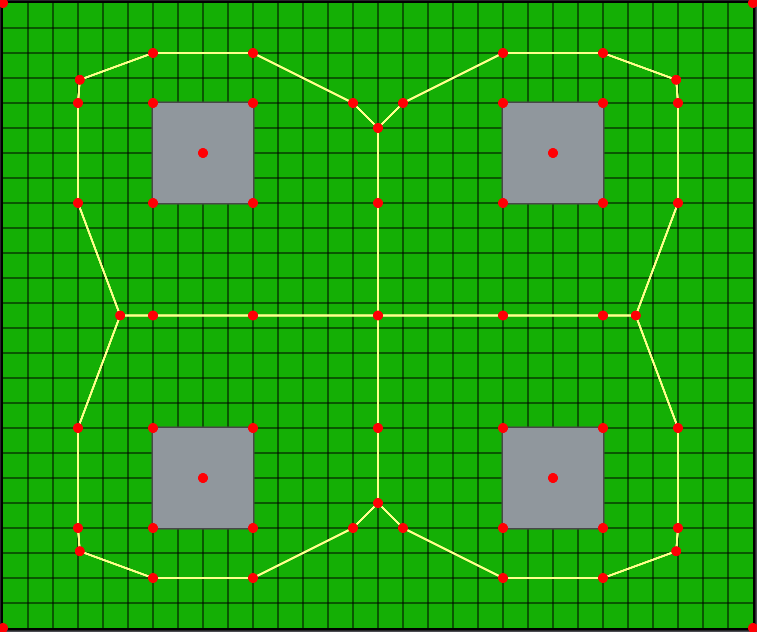
\includegraphics[scale=0.36]{voronoiGraphForMap}
\caption[Graf Voronoi dla mapy z przeszkodami przed powiększeniem]{Graf Voronoi dla mapy z przeszkodami przed powiększeniem}
\end{figure}

\newpage

\begin{figure}[h!]
\centering
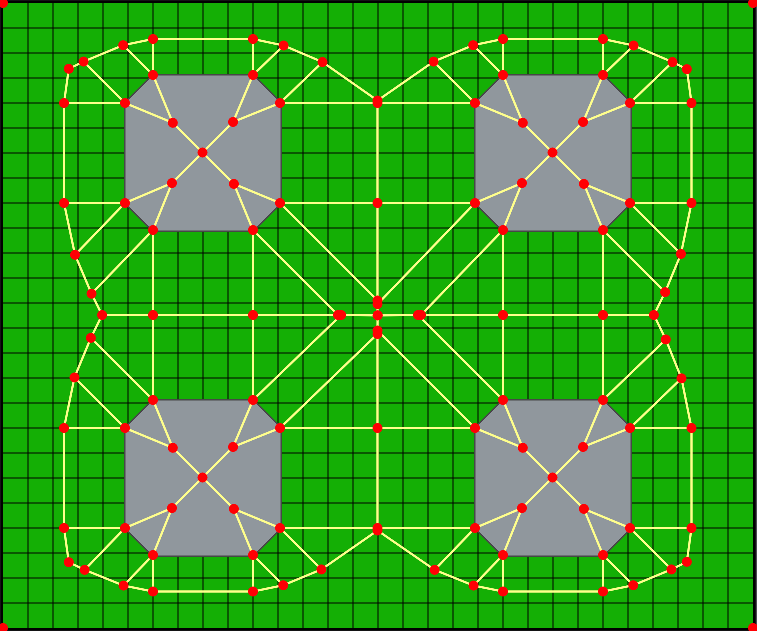
\includegraphics[scale=0.36]{voronoiGraphForExpandedMap}
\caption[Graf Voronoi dla mapy z przeszkodami po powiększeniu]{Graf Voronoi dla mapy z przeszkodami po powiększeniu}
\end{figure}

\subsubsection{Konstrukcja grafu i wyszukiwanie ścieżki}

Jak nie trudno się domyślić konstrukcja grafu, w którym wyszukiwana będzie ścieżka pomiędzy wierzchołkiem startowym i końcowym rozpoczyna się od wyznaczenia grafu Voronoi dla zadanej mapy (z powiększonymi przeszkodami lub nie). Ponieważ doświadczenia empiryczne pokazały, że sam graf Voronoi bardzo często zawiera zbyt mało wierzchołków i krawędzi, aby możliwe było wyznaczenie sensownej trajektorii dla pojazdu należało w jakiś sposób wzbogacić ten graf o nowe wierzchołki i krawędzie. Podstawowy pomysł polega na dodaniu krawędzi pomiędzy wszystkimi wierzchołkami, które są dla siebie nawzajem "widoczne", tzn. krawędź pomiędzy tymi wierzchołkami nie przechodzi przez żaden obiekt mapy (lub powiększony obiekt mapy). Przykładowy graf z dodatkowymi krawędziami przedstawia rysunek 5.4.

\begin{figure}[h!]
\centering
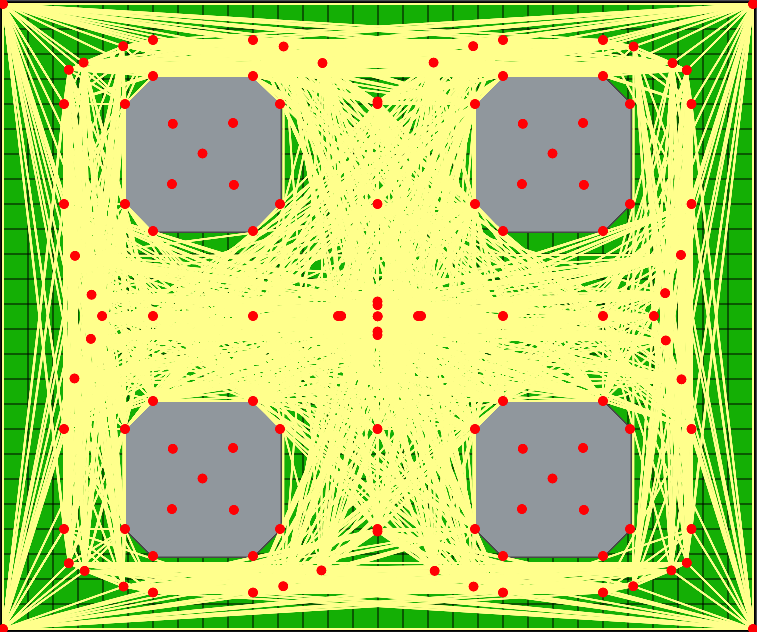
\includegraphics[scale=0.4]{fullVoronoiGraphForExpandedMap}
\caption[Graf Voronoi z dodatkowymi krawędziami]{Graf Voronoi z dodatkowymi krawędziami}
\end{figure}

W znakomitej większości przypadków taka modyfikacja grafu jest wystarczająca i pozwala na wyznaczenie sensownej trajektorii. Zdarzają się jednak sytuacje, w których okazuje się, że w grafie wyznaczonym powyższą metodą wciąż jest zbyt mało wierzchołków i krawędzi, żeby np. pojazd mógł się przecisnąć pomiędzy gęsto i ciasno rozlokowanymi przeszkodami. W tej sytuacji rozwiązaniem może być dodanie nowych, sztucznych wierzchołków oraz krawędzi pomiędzy tymi wierzchołkami, a wszystkimi wierzchołkami, dla których krawędź nie będzie kolidować z powiększonymi przeszkodami mapy. Graf będący wynikiem takiej operacji (dodane po 10 wierzchołków w pionie i w poziomie) przedstawiono na rysunku 5.5. Czytelność takiego grafu jest już jednak praktycznie zerowa, co wynika z ogromnej liczby krawędzi, które są tak gęsto rozmieszczone, iż niemal w całości pokrywają całą dostępną przestrzeń na mapie.

\begin{figure}[h!]
\centering
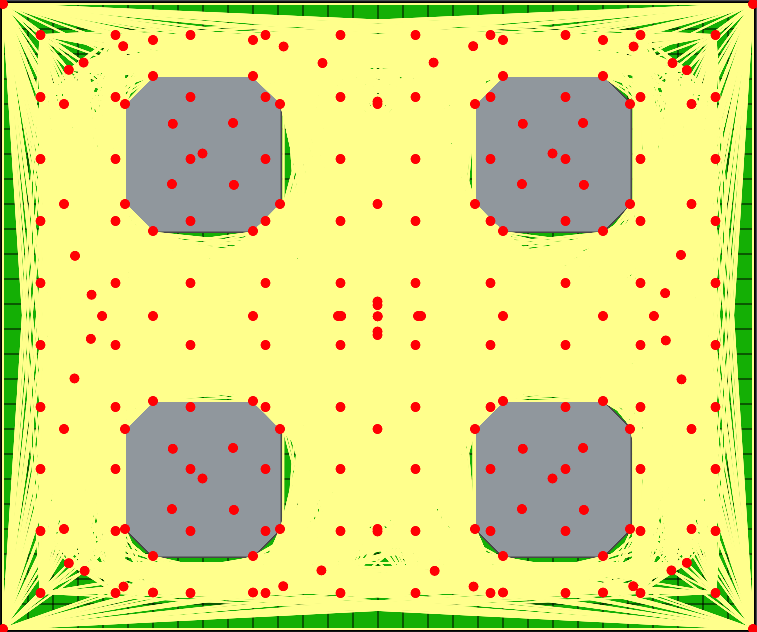
\includegraphics[scale=0.4]{fullVoronoiGraphForExpandedMapWithExtraVertices}
\caption[Graf Voronoi z dodatkowymi wierzchołkami i krawędziami]{Graf Voronoi z dodatkowymi wierzchołkami i krawędziami}
\end{figure}

Ostatnim krokiem w konstrukcji grafu jest dodanie do niego dwóch wierzchołków początkowych połączonych krawędzią (krawędź początkowa) oraz dwóch wierzchołków końcowych połączonych krawędzią (krawędź końcowa). Następnie należy połączyć końcowy wierzchołek krawędzi początkowej ze wszystkimi możliwymi wierzchołkami grafu. To samo należy zrobić z początkowym wierzchołkiem krawędzi końcowej. W tym momencie graf jest gotowy, aby przeprowadzić na nim wyszukiwanie ścieżki pomiędzy wierzchołkiem początkowym, a wierzchołkiem końcowym, np. przy pomocy algorytmu A*. Przykładową ścieżkę znalezioną w grafie dla pozycji startowej znajdującej się w lewym dolnym rogu mapy i pozycji końcowej znajdującej się w prawym górnym rogu mapy przedstawiono na rysunku 5.6.

\begin{figure}[h!]
\centering
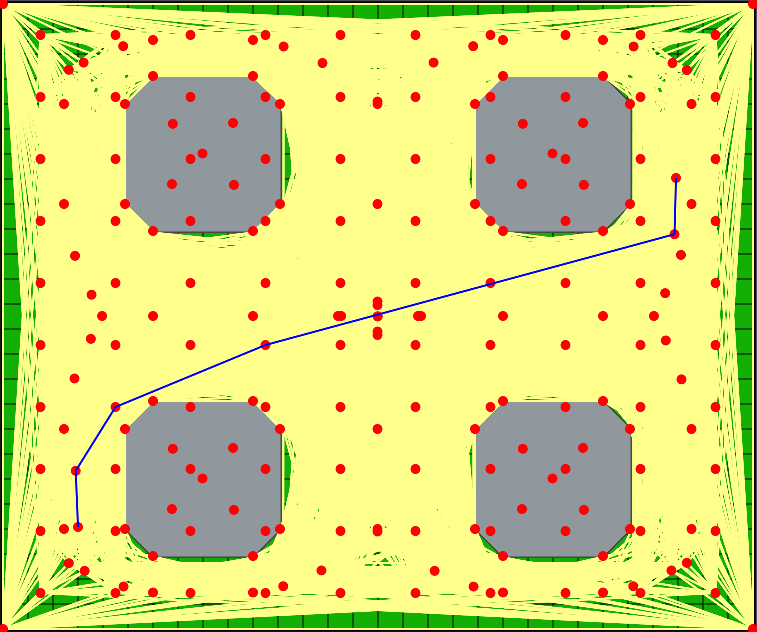
\includegraphics[scale=0.4]{polylinePathInVoronoiGraph}
\caption[Ścieżka wyznaczona w grafie pomiędzy położeniem początkowym i końcowym]{Ścieżka wyznaczona w grafie pomiędzy położeniem początkowym i końcowym}
\end{figure}

Poniżej przedstawiono również kompletny pseudokod procedury służącej do konstrukcji zmodyfikowanego grafu Voronoi wykorzystywanego przy planowaniu ruchu pojazdu pomiędzy zadanymi położeniami.

\begin{pseudokod}
Konstrukcja zmodyfikowanego grafu Voronoi
\begin{verbatim}
    wyznacz graf Voronoi dla dostarczonej mapy (np. za pomocą biblioteki Boost)
    jeśli liczba dodatkowych sztucznych wierzchołków jest niezerowa
        dodaj siatkę sztucznych wierzchołków do grafu
    dodaj do grafu dwa wierzchołki reprezentujące położenie początkowe i połącz je krawędzią
    dodaj do grafu dwa wierzchołki reprezentujące położenie końcowe i połącz je krawędzią
    dla każdej pary wierzchołków
        jeśli wierzchołki można połączyć bezkolizyjną krawędzią
            dodaj krawędź pomiędzy wierzchołkami do grafu
    zwróć wynikowy graf
\end{verbatim}
\end{pseudokod}

\subsubsection{Konstrukcja finalnej ścieżki za pomocą krzywej B-sklejanej}

Mając wyznaczoną łamaną, można przystąpić do jej ''poprawienia'' i konstrukcji na jej podstawie ścieżki, która będzie bardziej przyjazna dla pojazdu. Pierwszym proponowanym rozwiązaniem jest wykorzystanie krzywej B-sklejanej, która jest jedną z najczęściej stosowanych reprezentacji parametrycznych krzywych sklejanych. Krzywą B-sklejaną charakteryzują dwa parametry: 
\begin{itemize}
 \item \textbf{$n$} - stopień sklejanych krzywych wielomianowych (w przypadku niniejszej pracy stopień krzywych równy 3),
 \item \textbf{$m$} - liczba podprzedziałów, na których definiowane są kolejne części krzywej.
\end{itemize}

Krzywe B-sklejane, podobnie jak inne krzywe parametryczne używane w grafice komputerowej, są wyznaczane przez ciąg punktów kontrolnych $p_0, p_1, ..., p_{m-n+1}$. Krzywa taka jest reprezentowana przez $m - 2n$ krzywych wielomianowych stopnia $n$ (mówi się wówczas, że krzywa B-sklejana jest $n$-tego stopnia), które łączone są z określoną ciągłością parametryczną, zazwyczaj $C^{2}$.

Krzywa B-sklejana jest określona na przedziale $t \in [0, 1]$, natomiast ciąg $m + 1$ wartości $u_{i}$ dzieli ten przedział na podprzedziały, na których zdefiniowane są poszczególne krzywe wielomianowe. Wartości $u$ są nazywane węzłami krzywej (ang. \textit{knot}) i spełniają one zależność $u_{i} \leq u_{i+1}$, tzn. jest to niemalejący ciąg, a więc węzły mogą się powtarzać. Najczęściej zakłada się także, że $u_0 = 0$ oraz $u_{m} = 1$.

~\\Dowolny punkt na krzywej B-sklejanej jest dany następującym równaniem:
$$
p(t) = \sum_{i = 0}^{m - n - 1} p_{i} N^{n}_{i}(t) \quad dla \quad t \in [u_{n}, u_{m - n}],
$$
gdzie:
\begin{itemize}
	\item $m + 1$ - liczba węzłów,
	\item $n$ - stopień krzywej,
	\item $p_{i}$ - punkty kontrolne,
	\item $N^{n}_{i}(t)$ - unormowana funkcja B-sklejana stopnia $n$.
\end{itemize}

Na ogół unormowana funkcja B-sklejana jest przedstawiana za pomocą ilorazu różnicowego obciętych funkcji potęgowych, jednak forma ta jest dość skomplikowana i zamiast tego zapisujemy równoważny wzór rekurencyjny Mansfielda-de Boora-Coxa, będący podstawą algorytmu de Boora:
\\
$$
N^{0}_{i}(t) = 
\left\{ \begin{array}{ll}
1 & \textrm{dla $t \in [u_{i}, u_{i+1})$}\\
0 & \textrm{w przeciwnym wypadku}
\end{array} \right.
$$
$$
N^{n}_{i}(t) = \frac{t - u_{i}}{u_{i + n} - u{i}}N^{n - 1}_{i}(t) + \frac{u_{i + n + 1} - t}{u_{i + n + 1} - u{i + 1}}N^{n - 1}_{i + 1}(t) \quad dla \quad n > 0.
$$
\\
Wszystkie krzywe składowe leżą w otoczce wypukłej swoich punktów kontrolnych, stąd cała krzywa B-sklejana leży w obszarze będącym sumą otoczek. Przykład przedstawiono na rysunku 5.7.

\begin{figure}[h!]
\centering
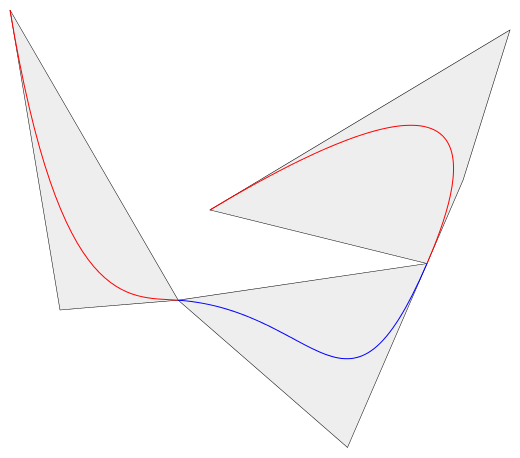
\includegraphics[scale=0.3]{bsplineConvexHull}
\caption[Przykładowa krzywa B-Sklejana]{Przykładowa krzywa B-sklejana}
\end{figure}

Mając zdefiniowaną krzywą B-sklejaną oraz opisany sposób obliczania jej kolejnych punktów można teraz wykorzystać ją do konstrukcji trajektorii, po której będzie poruszał się pojazd. W tym celu należy wziąć wszystkie wierzchołki wchodzące w skład wyznaczonej w poprzednich krokach łamanej i potraktować je jako punkty kontrolne krzywej B-sklejanej. Następnie należy wykonać obliczenia wszystkich punktów krzywej i w ten prosty sposób wyznaczona zostaje finalna trajektoria. Przykład krzywej wyznaczonej dla łamanej z poprzedniego podrozdziału przedstawia rysunek 5.8.

\begin{figure}[h!]
\centering
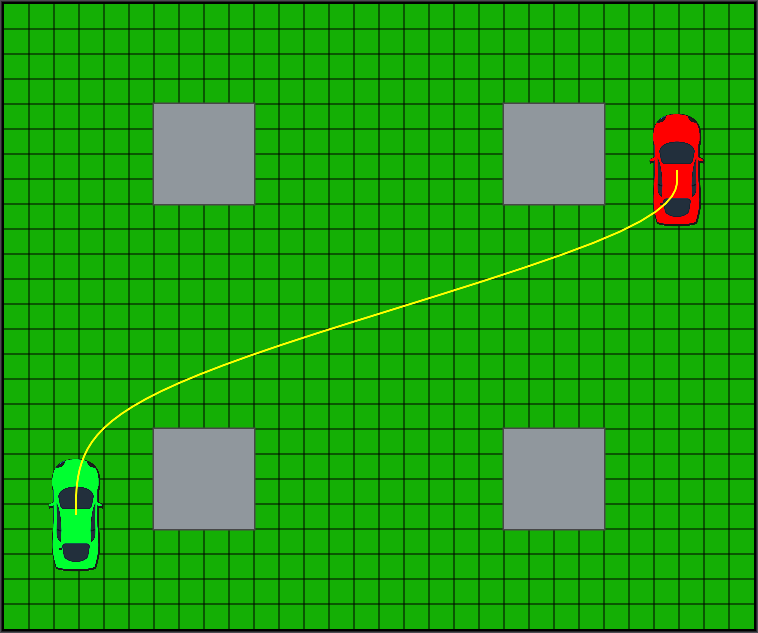
\includegraphics[scale=0.4]{finalPathBSpline}
\caption[Trajektoria skonstruowana z wykorzystaniem krzywej B-sklejanej]{Trajektoria skonstruowana z wykorzystaniem krzywej B-sklejanej}
\end{figure}

Zastosowanie krzywej B-sklejanej do konstrukcji ścieżki dla pojazdu jest rozwiązaniem stosunkowo prostym. Jedyne trudności jakie pojawiły się przy implementacji tej metody to zaimplementowanie wszystkich procedur niezbędnych do obliczania punktów na krzywej, takich jak np. algorytm De Boora. Jednak mając już gotową obsługę krzywych B-sklejanych wystarczy przekazywać do algorytmu odpowiednie punkty kontrolne i natychmiast generowana jest wynikowa trajektoria. Rozwiązanie to nie jest jednak idealne, gdyż zdarzają się sytuacje, w których krzywa zbyt mocno oddala się od wyznaczonej łamanej, przez co zwiększa się ryzyko kolizji pojazdu z przeszkodami na mapie. Kolejnym problemem jest generowanie zbyt ostrych zakrętów, które w praktyce są nieosiągalne dla pojazdu o ograniczonej skrętności kół. Z uwagi na wymienione wady tej metody zaimplementowana została jeszcze jedna metoda generowanie trajektorii na podstawie łamanej, tym razem oparta na wpisywaniu łuków pomiędzy kolejne odcinki łamanej. Metoda ta została opisana w kolejnym punkcie tego rozdziału.

\subsubsection{Konstrukcja finalnej ścieżki za pomocą wpisywania łuków pomiędzy odcinki łamanej}

W tej części omówiony zostanie algorytm konstrukcji trajektorii na podstawie zadanej łamanej poprzez wpisywanie łuków pomiędzy kolejne odcinki łamanej. Powodem rozważania tej metody jest próba eliminacji zbyt ostrych łuków jakie są generowane podczas wyznaczania ścieżki za pomocą krzywej sklejanej.

Na początek załóżmy, że jako dane wejściowe mamy trzy punkty, czyli dwa odcinki o wspólnym wierzchołku. Zadaniem algorytmu będzie wyznaczenie parametrów łuku niezbędnych do tego, aby gładko wstawić taki łuk pomiędzy te odcinki. 

\begin{figure}[h!]
\centering
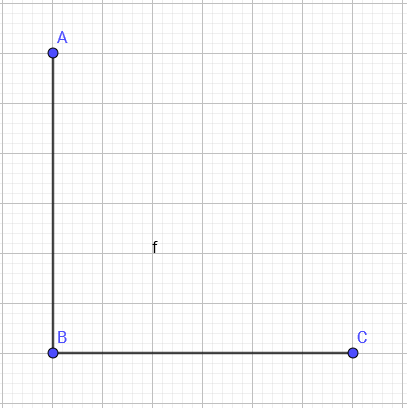
\includegraphics[scale=0.35]{arcsAlgorithmStep1}
\caption[Dane wejściowe dla algorytmu wpisywania łuku pomiędzy odcinki]{Dane wejściowe dla algorytmu wpisywania łuku pomiędzy odcinki}
\end{figure}

Aby móc wpisać łuk pomiędzy zadane odcinki należy wyznaczyć środek okręgu, do którego należy dany łuk, kąt początkowy oraz kąt końcowy, a także kierunek łuku - zgodny lub przeciwny do ruchu wskazówek zegara, w skrócie CW lub CCW. Wyznaczenie wymienionych parametrów łuku odbywa się w następujących krokach:
\begin{itemize}
	\item wyznaczenie wektorów kierunku i długości odcinków pomiędzy które chcemy wpisać okrąg - jest to operacja trywialna, oznaczmy jej wyniki jako: $dir(B,A), dir(C,B), len(B,A), len(C,B)$,
	\item wyznaczenie wektorów normalnych do odcinków $BA$ oraz $CB$. Można to zrobić w następujący sposób:
	$$normal(B,A) = [dir(B,A).y, -dir(B,A).x]$$
	$$normal(C,B) = [dir(C,B).y, -dir(C,B).x]$$
	\item pobranie minimalnego promienia skrętu, który jest dozwolony dla danego pojazdu - $r_{min}$,
	\item umieszczenie dwóch punktów $P$ i $K$ na dwóch odcinkach w odległości od punktu $B$ równej długości dłuższej krawędzi ($length$). W zaprezentowanym przykładzie złożyło się tak, iż pokrywają się one z punktami $A$ i $C$, ponieważ oba odcinki są równej długości,
	\item wyznaczanie środka okręgu oraz iteracyjne ściąganie punktów $P$ i $K$ w kierunku punktu $B$ do momentu, aż promień okręgu nie osiągnie wartości minimalnego promienia dla danego pojazdu. Poniżej zaprezentowano obliczenia i rysunek przedstawiający opisaną sytuację:
	$$P = B - length * dir(B,A)$$
	$$K = B + length * dir(C,B)$$
	$$P_{1} = P$$
	$$P_{2} = P + normal(B,A)$$
	$$P_{3} = K$$
	$$P_{4} = K + normal(C,B)$$
	$$CENTER = IntersectPoint(P_{1}, P_{2}, P_{3}, P_{4})$$

\begin{figure}[h!]
\centering
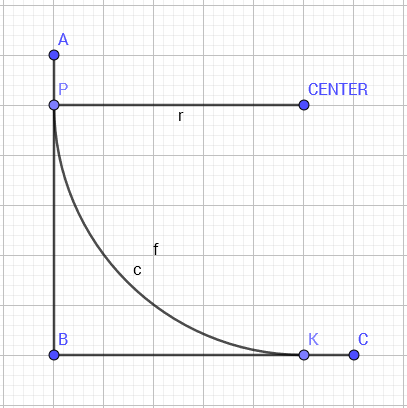
\includegraphics[scale=0.35]{arcsAlgorithmStep2}
\caption[Dane wejściowe dla algorytmu wpisywania łuku pomiędzy odcinki]{Dane wejściowe dla algorytmu wpisywania łuku pomiędzy odcinki}
\end{figure}

	\item sprawdzenie czy łuk jest CW, czy CCW za pomocą dowolnego algorytmu geometrycznego, który określi kierunek odcinków $AB$ oraz $BS$,
	\item wyznaczenie kąta początkowego i końcowego poprzez sprawdzenie kąta nachylenia odcinków $AB$ oraz $BC$.

\end{itemize}

Po wykonaniu wszystkich opisanych powyżej kroków wyznaczone zostaną wszystkie parametry opisujące łuk wpisany pomiędzy dwa odcinki. Poniżej przedstawiono pseudokod całej procedury.

\begin{pseudokod}
Wpisywanie łuku pomiędzy dwa odcinki
\begin{verbatim}
    AB, BC - dwa wejściowe odcinki o wspólnym wierzchołku
    l1 = len(B,A)
    l2 = len(C,B)
    dir1 = dir(B,A)
    dir2 = dir(C,B)
    n1 = [dir1.y, -dir1.x]
    n2 = [dir2.y, -dir2.x]
    length = l1 > l2 ? l1 : l2
    radiusMin = minimalny promień skrętu pojazdu
    radius = +INF
    dopóki radius > radiusMin
        P = B + length * dir1
        K = B + length * dir2
        P1 = P
        P2 = P + n1
        P3 = K
        P4 = K + n2
        CENTER = znajdź punkt przecięcia odcinków P1P2 oraz P3P4
        radius = length(P, CENTER)  
        length -= 0.1
    kierunekŁuku = kierunek wzajemny odcinków AB i BC
    kątStartowy = kąt nachylenia odcinka AB
    kątKońcowy = kąt nachylenia odcinka BC
    zwróć łuk(CENTER, kątStartowy, kątKońcowy, kierunekŁuku)
\end{verbatim}
\end{pseudokod}

Znając metodę wyznaczania parametrów łuku wpisanego pomiędzy dwa odcinki można przedstawić kompletny algorytm konstrukcji finalnej trajektorii na podstawie łamanej. Tutaj sprawa jest dość prosta, ponieważ tak naprawdę wystarczy wyznaczyć listę łuków wpisanych pomiędzy każdą parę odcinków, a następnie pomiędzy każdą parę łuków wstawić linię łącząca końcowy punkt pierwszego łuku z początkowym punktem drugiego łuku. Ponadto należy dodać linie łączące punkt startowy z punktem początkowym pierwszego łuku na liście oraz linię łączącą końcowy punkt ostatniego łuku z listy z punktem końcowym. Całość procedury przedstawia poniższy pseudokod.

\begin{pseudokod}
Wyznaczanie trajektorii opartej na wpisywanych łukach
\begin{verbatim}
    finalna ścieżka = pusta
    dla każdej pary odcinków
        wyznacz parametry łuku wpisanego pomiędzy te odcinki i dodaj go 
        do finalnej ścieżki
    dla każdej pary łuków znajdujących się w finalnej ścieżce
        dodaj linię do finalnej ścieżki, która łączy koniec jednego łuku 
        z początkiem drugiego
    dodaj linię łączącą punkt początkowy z pierwszym punktem pierwszego łuku w 
    finalnej ścieżce
    dodaj linię łączącą punkt końcowy z ostatnim punktem ostatniego łuku w finalnej ścieżce
    zwróć finalną ścieżkę
\end{verbatim}
\end{pseudokod}

Przykładowa ścieżka wygenerowana z łamanej z poprzedniego rozdziału przy zastosowaniu algorytmu wpisywania łuków została przedstawiona na rysunku 5.11.

\begin{figure}[h!]
\centering
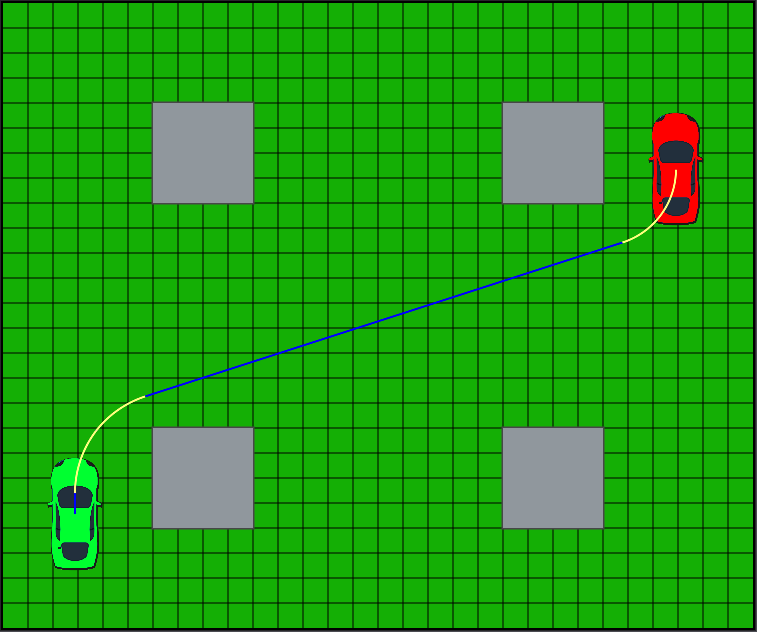
\includegraphics[scale=0.4]{finalPathArcs}
\caption[Trajektoria skonstruowana z wykorzystaniem metody wpisywania łuków]{Trajektoria skonstruowana z wykorzystaniem metody wpisywania łuków}
\end{figure}

\subsubsection{Wykrywanie i eliminacja kolizji}

W zaimplementowanej aplikacji mechanizm wykrywania i eliminacji kolizji może zostać w dowolnym momencie włączony lub wyłączony przez użytkownika oraz to użytkownik określa jego dokładność. Jak nietrudno się domyślić wraz ze wzrostem dokładności wykrywania kolizji i ich eliminacji wzrasta też ilość czasu, która jest potrzebna na wykonanie niezbędnych obliczeń. 

Sam proces wykrywania kolizji jest dość prosty. Idea jest taka, że symulujemy ruch pojazdu po wyznaczonej w poprzednich krokach trajektorii uaktualniając jego stan do stanu jaki miałby znajdując się w danym punkcie ścieżki. Następnie algorytm sprawdza, czy występuje kolizja pojazdu z którąś z przeszkód znajdujących się na mapie. Jeśli nie, to wszystko jest w porządku i sprawdzane jest kolejne położenie. Jeśli natomiast kolizja wystąpiła, to odnajdywana jest krawędź grafu, która z największym prawdopodobieństwem odpowiada za kształt danego fragmentu ścieżki i następuje usunięcie tej krawędzi z grafu. Następnie wyznaczana jest nowa trajektoria i cały proces zaczyna się od początku. Liczba punktów ścieżki dla których sprawdzana jest kolizja pojazdu z przeszkodami jest definiowana przez użytkownika i od liczby tych punktów zależy jakość i czas działania algorytmu wykrywania i eliminacji kolizji. Dla uporządkowania poniżej przedstawiono pseudokod opisanego algorytmu.

\newpage

\begin{pseudokod}
Wykrywanie i eliminacja kolizji
\begin{verbatim}
    dla określonej przez użytkownika liczby położeń pojazdu na ścieżce
        zaktualizuj stan pojazdu do określonego położenia na ścieżce
        sprawdź kolizję pojazdu z przeszkodami znajdującymi się na mapie
        jeśli nie występuje kolizja
            kontynuuj
        w przeciwnym wypadku
            znajdź krawędź w grafie, która odpowiada za dany fragment 
            wynikowej ścieżki
            usuń znalezioną krawędź z grafu
            wyznacz na nowo ścieżkę i rozpocznij proces wykrywania i eliminacji 
            kolizji od początku
\end{verbatim}
\end{pseudokod}

\subsection{Pseudokod algorytmu planowania ruchu}

W tym podrozdziale przedstawiony zostanie kompletny pseudokod algorytmu planowania ruchu pojazdu pomiędzy punktem początkowym, a końcowym.

\begin{pseudokod}
Algorytm planowania ruchu
\begin{verbatim}
    jeśli pozycja początkowa znajduje się w miejscu parkingowym
        wyznacz ścieżkę wyjazdową i jako punkt początkowy przyjmij 
        jej ostatni punkt
    jeśli pozycja końcowa znajduje się w miejscu parkingowym
        wyznacz ścieżkę wjazdową i jako punkt końcowy przyjmij 
        jej pierwszy punkt
    powiększ przeszkody znajdujące się na mapie zgodnie z parametrami użytkownika
    utwórz graf Voronoi lub zmodyfikowany graf Voronoi w zależności od 
    parametrów dostarczonych przez użytkownika
    wyznacz ścieżkę w utworzonym grafie pomiędzy punktem początkowy, 
    a punktem końcowym wykorzystując jeden z algorytmów wyszukiwania 
    ścieżki w grafie np. algorytm A*
    dopóki włączona jest detekcja kolizji i występuje kolizja lub jest to pierwszy 
    obrót pętli
        jeżeli wybrano algorytm wykorzystujący krzywą B-sklejaną
            wyznacz finalną trajektorię korzystając z algorytmu wykorzystującego 
            krzywą B-sklejaną
        w przeciwnym wypadku
            wyznacz finalną trajektorię korzystając z algorytmu wpisywania łuków
             pomiędzy odcinki łamanej
        jeśli występuje kolizja na wyznaczonej ścieżce
            usuń kolizję algorytmem wykrywania i eliminacji kolizji
        w przeciwnym wypadku
            przerwij pętlę
    zwróć finalną ścieżkę
\end{verbatim}
\end{pseudokod}

\subsection{Testy i dalszy rozwój algorytmu}

Pierwszym, podstawowym testem algorytmu planowania ruchu jest sprawdzenie jaka trajektoria zostanie wyznaczona przy zwyczajnym poruszaniu się pojazdu do przodu. Test przebiegł oczywiście pomyślnie, a wygenerowana została trajektoria przedstawiona na poniższym obrazku.

\begin{figure}[h!]
\centering
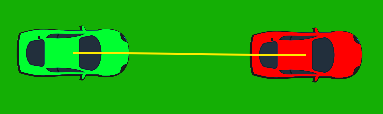
\includegraphics[scale=0.9]{simplePath0}
\caption[Trajektoria ruchu w przód]{Trajektoria ruchu w przód}
\end{figure}

Kolejnym testem było sprawdzenie, jakie trajektorie wygenerują oba typy algorytmu dla przejazdu pojazdu na miejsce obok pierwotnego miejsca postoju zarówno ze zmianą jak i bez zmiany orientacji. Ścieżki otrzymane dla algorytmu wykorzystującego krzywe B-sklejane przedstawione zostały na obrazku 5.13, zaś ścieżki wygenerowane metodą wpisywanych łuków na obrazku 5.14.

\begin{figure}[h!]
\centering
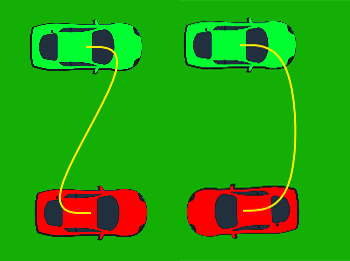
\includegraphics[scale=0.9]{simplePath1}
\caption[Proste ścieżki wygenerowane przy użyciu krzywej sklejanej]{Proste ścieżki wygenerowane przy użyciu krzywej sklejanej}
\end{figure}

\begin{figure}[h!]
\centering
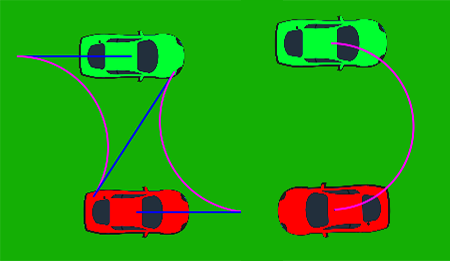
\includegraphics[scale=0.9]{simplePath2}
\caption[Proste ścieżki wygenerowane przy użyciu metody wpisanych łuków]{Proste ścieżki wygenerowane przy użyciu metody wpisanych łuków}
\end{figure}

Na pierwszy rzut oka ścieżki wygenerowane przy pomocy krzywej B-sklejanej wyglądają bardziej elegancko, jednak po uważnym spojrzeniu na pierwszą trajektorię przemieszczenia pojazdu bez zmiany jego orientacji nietrudno zauważyć, że zakręty na początku i na końcu ścieżki są zbyt ostre i w praktyce nieosiągalne dla prawdziwego samochodu. Jeśli jednak zaniedbamy chwilowo osiągalność poszczególnych skrętów, to ścieżki te są jak najbardziej poprawne i w dodatku są one zgodne z oczekiwaniami.

Ścieżki, które zostały przedstawione na drugim obrazku nie wyglądają z pozoru już tak dobrze, w szczególności pierwsza z nich, która swoim kształtem może wydawać się dość zaskakująca. Jak się jednak okazuje ścieżka ta jest w pełni poprawna, a pojazd o maksymalnym skręcie kół około 45 stopni jest w stanie ją pokonać w rzeczywistości. Ścieżka ta ukazuje jednak problem jaki będzie się pojawiał podczas korzystania z algorytmu wpisywanych łuków, a dotyczy on sytuacji, w których krawędzie pomiędzy które wpisany ma zostać łuk są zbyt krótkie. W takiej sytuacji krawędź taka jest sztucznie wydłużana, co powoduje, że pomiędzy kolejnymi łukami mogą pojawiać się odcinki, po których pojazd będzie zmuszony przejechać do tyłu, aby z końca jednego łuku dostać się na początek następnego. Opisana sytuacja została w pełni zobrazowana na rysunku 5.15.

\begin{figure}[h!]
\centering
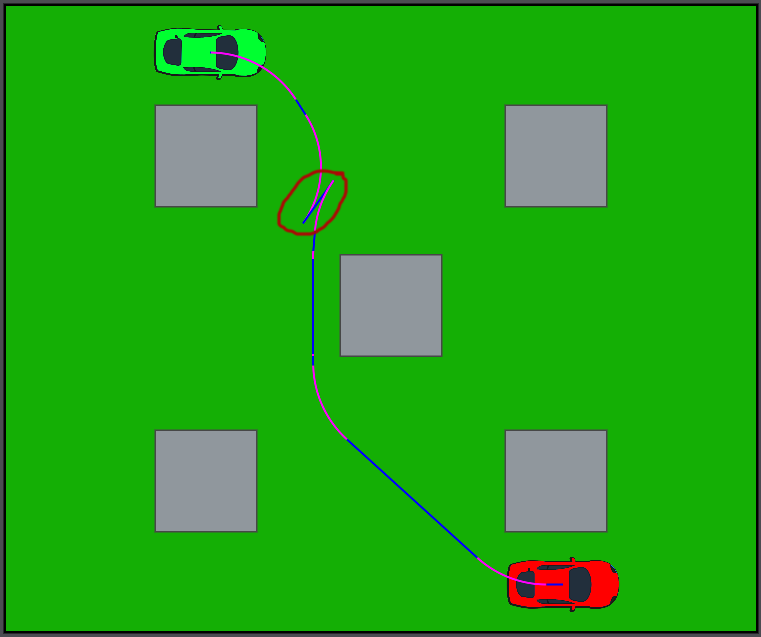
\includegraphics[scale=0.6]{simplePath3}
\caption[Proste ścieżki wygenerowane przy użyciu metody wpisanych łuków]{Proste ścieżki wygenerowane przy użyciu metody wpisanych łuków}
\end{figure}

W przykładzie tym mamy do czynienia z klasycznym problemem, jaki występuje w metodzie wpisanych łuków. Widać, że w zaznaczonym obszarze łuki powinny się spotkać swoimi końcami, jednak było tam zbyt ciasno, przez co krawędzie musiały zostać przedłużone i doszło do sytuacji, że pojazd aby przedostać się z jednego łuku na drugi musi wykonać ruch do tyłu. Mimo iż ścieżka ta wydaje się bardzo nieelegancka i w praktyce pewnie nigdy pojazd nie powinien się tak zachowywać, to jednak wciąż jest to poprawna ścieżka, która pozwala na bezkolizyjny ruch pojazdu pomiędzy zadanymi położeniami, a na dodatek wszystkie zakręty, które pojazd wykonuje podczas ruchu są dla niego osiągalne w rzeczywistości, przy zadanym maksymalnym skręcie kół.

Poza dość prostymi testami jak te zaprezentowane powyżej zostały przeprowadzone również testy na dużo bardziej skomplikowanych mapach. W większości przypadków zakończyły się one pomyślnie i została wygenerowana mniej lub bardziej sensowna z punktu widzenia zwykłego człowieka trajektoria dla pojazdu. Zdarzały się jednak przypadki, iż ścieżka nie była wyznaczana i konieczne było dodanie określonej liczby sztucznych wierzchołków w sytuacji, w której na pierwszy rzut oka taka ścieżka powinna zostać wyznaczona bez większych problemów. Takie zachowanie algorytmu wynika z faktu, iż cały proces wyznaczania ścieżki jest determinowany poprzez położenie wierzchołków grafu i przy niefortunnym ułożeniu przeszkód wierzchołki mogą zostać tak rozmieszczone, że niemożliwa jest konstrukcja ścieżki bezkolizyjnej opartej na dowolnej łamanej złożonej z krawędzi takiego grafu. Dodanie sztucznych wierzchołków na ogół eliminowało takie problemy, ale w zamian za to czas obliczeń znacząco wzrastał. Na ostatnim już obrazku w tym podrozdziale została przedstawiona ścieżka dla bardziej skomplikowanej mapy - rysunek 5.16.

\newpage

\begin{figure}[h!]
\centering
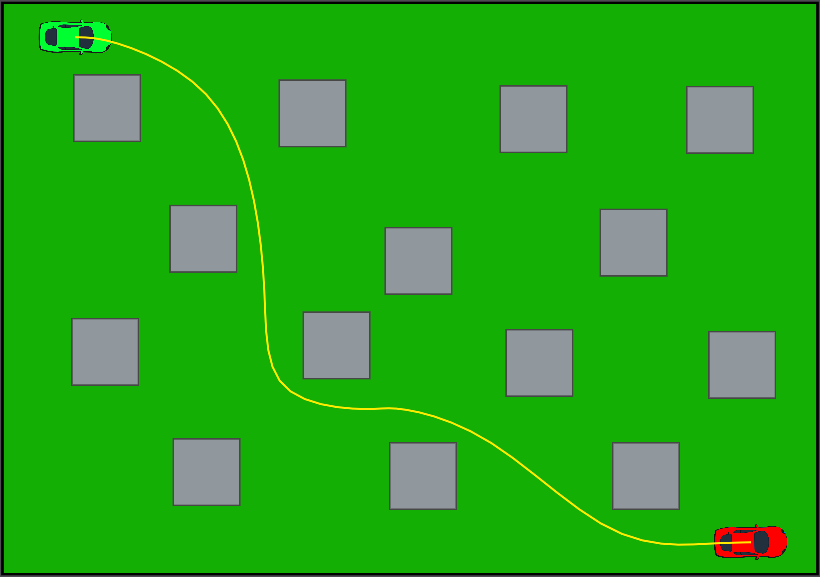
\includegraphics[scale=0.65]{simplePath4}
\caption[Proste ścieżki wygenerowane przy użyciu metody wpisanych łuków]{Proste ścieżki wygenerowane przy użyciu metody wpisanych łuków}
\end{figure}

Jak pokazały przeprowadzone testy algorytm działa poprawnie i potrafi wyznaczyć ścieżkę nawet w dość skomplikowanym przypadku. Zdarzają się jednak sytuacje, w których ścieżka nie zostaje znaleziona, choć patrząc na mapę od razu widać, że istnieje. W takich przypadkach najczęściej wystarczy zmienić parametry wyszukiwania ścieżki i dodać dodatkowe wierzchołki do konstruowanego grafu. Kolejnym etapem rozwoju algorytmu mogłaby być automatyzacja tego procesu i automatyczny dobór parametrów przez algorytm w zależności od wczytanej przez użytkownika mapy.

Kolejne problemy jakie ujawniły testy to dodawanie krawędzi wstecznych w metodzie wpisywania łuków oraz długi czas obliczeń dla bardziej skomplikowanych map, gdy włączony jest algorytm wykrywania i eliminacji kolizji pojazdu z przeszkodami. Pokrywa się to jednak z przewidywaniami, ponieważ algorytm wykrywania i eliminacji kolizji jest  procesem dość kosztownym i gdy układ przeszkód na mapie wymusza jego intensywne użycie to czas obliczeń znacząco rośnie. Rozwiązanie wymienionych problemów i optymalizacja algorytmu byłaby celem kolejnego etapu prac nad planerem ruchu, gdyby do niego doszło.

\newpage

\subsection{Wpływ parametrów algorytmu na czas obliczeń}

W tej części dokumentu zaprezentowany zostanie wpływ następujących parametrów na czas działania algorytmu:
\begin{itemize}
	\item gęstości siatki sztucznych wierzchołków dodanych do grafu,
	\item jakości algorytmu wykrywania i eliminacji kolizji.
\end{itemize}

Wpływ tych parametrów na czas obliczeń został przebadany empirycznie. Doświadczenia pokazały również, że pozostałe parametry konfigurowane przez użytkownika takie jak wartość procentowa szerokości pojazdu o jaką powiększane są przeszkody oraz wybór pomiędzy algorytmem opartym na krzywej B-sklejanej lub wpisywanych łukach nie mają większego wpływu na czas obliczeń tylko na jakość lub w ogóle istnienie ścieżki.

Wszystkie czasy działania algorytmu zostały uśrednione - wykonanych zostało po 5 prób dla każdego zestawu parametrów i danych wejściowych, a następnie wyliczono średnią arytmetyczną z tych prób i ta wartość została zapisana. Wyniki pomiarów zostały w dalszej części zapisane w tabelach oraz zaprezentowane w postaci wykresów.

Dla niezbyt skomplikowanych i średnio skomplikowanych map (do 25-30 przeszkód) czas obliczeń jest zadowalający. Jednak w przypadku bardziej skomplikowanych map, gdzie liczba przeszkód jest już bardzo duża, czas działania algorytmu znacząco się wydłuża. Jest to zdeterminowane głównie złożonością zaprojektowanego algorytmu wykrywania i eliminacji kolizji (gdy układ przeszkód na mapie powoduje jego intensywne wykorzystanie), a także wybranym podejściem do konstrukcji grafu, na podstawie którego konstruowana jest finalna ścieżka dla pojazdu.

\subsubsection{Wpływ gęstości siatki sztucznych wierzchołków dodanych do grafu na czas obliczeń}

Poniżej zaprezentowano wpływ gęstości siatki sztucznie dodanych wierzchołków w grafie (w którym następnie wyszukiwana jest łamana na podstawie której konstruowana jest finalna ścieżka) na czas działania algorytmu planowania ruchu. Mapa na której przeprowadzano testy zawierała 20 przeszkód, ale gwarantowała istnienie ścieżki pomiędzy położeniem początkowym i końcowym. Pomiary zostały wykonane dla następujących danych i parametrów:
\begin{itemize}
	\item procent powiększenia przeszkód: 50,
	\item algorytm planowania ruchu: krzywa B-sklejana,
	\item jakość algorytmu wykrywania i eliminacji kolizji: wyłączony.
\end{itemize}

\begin{table}[!h]
\begin{center}
	\begin{tabular}{ c c }
		\begin{tabular}{ | c | c | }
    \hline
    \textbf{Gęstość siatki} & \textbf{Czas obliczeń [ms]} \\
    \textbf{dodatkowych} &  \\
    \textbf{wierzchołków} &  \\ \hline
    	0 &	1146 \\ \hline
		1 &	1154 \\ \hline
		2 &	1172 \\ \hline
		3 &	1198 \\ \hline
		4 &	1234 \\ \hline
		5 &	1284 \\ \hline
		6 &	1339 \\ \hline
		7 &	1440 \\ \hline
	\end{tabular} &
	\begin{tabular}{ | c | c | }
    \hline
    \textbf{Gęstość siatki} & \textbf{Czas obliczeń [ms]} \\
    \textbf{dodatkowych} &  \\
    \textbf{wierzchołków} &  \\ \hline
		8 &	1485 \\ \hline
	9 &	1586 \\ \hline
	10 &	1729 \\ \hline
	11 &	1833 \\ \hline
	12 &	2033 \\ \hline
	13 &	2190 \\ \hline
	14 &	2344 \\ \hline
	15 &	2560 \\ \hline
 	\end{tabular}
	\end{tabular}\\
\end{center}
\caption{Wpływ gęstości siatki sztucznych wierzchołków dodanych do grafu na czas obliczeń}
\end{table}

\begin{figure}[h!]
\centering
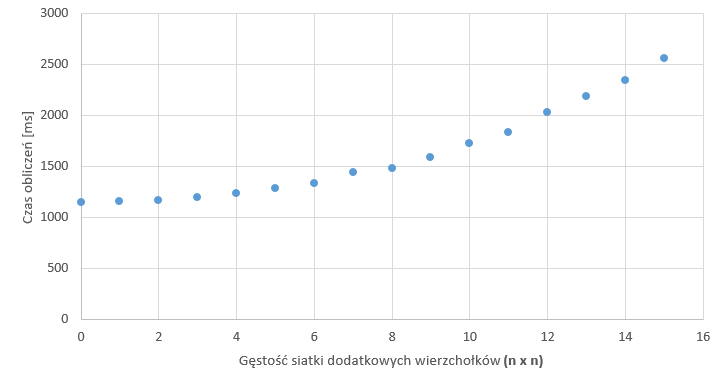
\includegraphics[scale=0.8]{chartExtraVertices}
\caption[Wpływ ilości sztucznych wierzchołków dodanych do grafu na czas obliczeń]{Wpływ gęstości siatki sztucznych wierzchołków dodanych do grafu na czas obliczeń}
\end{figure}

\subsubsection{Wpływ jakości wykrywania i eliminacji kolizji na czas obliczeń}

Poniżej zaprezentowano wpływ parametru określającego jakość działania algorytmu wykrywania i eliminacji kolizji podczas wyznaczania ścieżki dla pojazdu. Parametr ten może przyjmować wartość od 0 do 100, gdzie 0 oznacza brak jakiegokolwiek sprawdzania kolizji pojazdu z przeszkodami na mapie, natomiast 100 oznacza najlepszy wariant i najbardziej dokładne obliczenia. W tym wypadku, aby w ogóle można było mierzyć czas potrzebny na sprawdzanie kolizji, na mapie znajdowało się 15 przeszkód. Pomiary zostały wykonane dla następujących danych i parametrów:
\begin{itemize}
	\item procent powiększenia przeszkód: 50%,
	\item algorytm planowania ruchu: krzywa B-sklejana,
	\item gęstość siatki sztucznie dodawanych wierzchołków do grafu: 0.
\end{itemize}

\begin{table}[!h]
\begin{center}
	\begin{tabular}{ c c }
		\begin{tabular}{ | c | c | }
    \hline
    \textbf{Jakość wykrywania} & \textbf{Czas obliczeń [ms]} \\
    \textbf{i eliminacji} &  \\
    \textbf{kolizji} &  \\ \hline
    	0 &	1146 \\ \hline
		10 &	1139 \\ \hline
		20 &	1838 \\ \hline
		30 &	2347 \\ \hline
		40 &	2398 \\ \hline
		50 &	2466 \\ \hline
	\end{tabular} &
	\begin{tabular}{ | c | c | }
    \hline
    \textbf{Jakość wykrywania} & \textbf{Czas obliczeń [ms]} \\
    \textbf{i eliminacji} &  \\
    \textbf{kolizji} &  \\ \hline
		60 &	2564 \\ \hline
		70 &	2701 \\ \hline
		80 &	2698 \\ \hline
		90 &	2777 \\ \hline
		100 &	2785 \\ \hline
  	\end{tabular}
	\end{tabular}\\
  \caption{Wpływ jakości wykrywania i eliminacji kolizji na czas obliczeń}
\end{center}
\end{table}

\begin{figure}[h!]
\centering
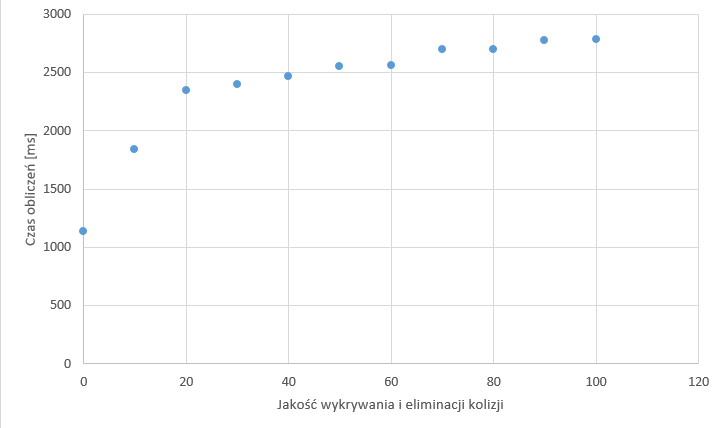
\includegraphics[scale=0.8]{chartCollisionDetectionQuality}
\caption[Wpływ jakości wykrywania i eliminacji kolizji na czas obliczeń]{Wpływ jakości wykrywania i eliminacji kolizji na czas obliczeń}
\end{figure}

Wyniki doświadczeń przeprowadzonych dla jakości działania algorytmu wykrywania i eliminacji kolizji są dość zaskakujące. Okazało się, że wpływ działania tego algorytmu na czas obliczeń jest ściśle związany z układem przeszkód na mapie. Dla testowej mapy już słaba jakość algorytmu (10 - 20) pozwalała na wykrycie i eliminację wszystkich kolizji i zwiększanie jakości nie powodowało znacznego wydłużania czasu obliczeń. Gdy jednak mapa jest bardziej skomplikowana a ścieżka trudna do wyznaczenia to algorytm ten może zacząć zachowywać się w zupełnie inny sposób i wówczas to jego złożoność będzie miała główny wpływ na czas działania całego algorytmu planowania ruchu. 

\newpage

\section{Algorytm parkowania}

W tym podrozdziale opisany zostanie algorytm, który umożliwi zaparkowanie pojazdu zarówno w miejscu przeznaczonym do parkowania równoległego jak i prostopadłego. Zanim jednak opisany zostanie sam algorytm dokonana zostanie geometryczna analiza problemu parkowania równoległego.

\subsection{Analiza problemu parkowania równoległego}

Podczas próby zaparkowania równoległego pojazdu w wybranym miejscu parkingowym możliwe jest wystąpienie jednej z wymienionych poniżej sytuacji:
\begin{itemize}
	\item miejsce parkingowe jest za małe i zaparkowanie pojazdu w ogóle nie jest możliwe,
	\item miejsce parkingowe jest wystarczającej wielkości aby pojazd się w nim zmieścił, ale wymaga wykonania kilku ruchów w przód i w tył.	
	\item miejsce parkingowe jest dostatecznie duże i możliwe jest zaparkowanie w jednym manewrze,
\end{itemize}

Oczywiście przy definiowaniu powyższych przypadków nie są brane pod uwagę dodatkowe ograniczenia, które mogą wystąpić w otoczeniu miejsca parkingowego i np. uniemożliwić parkowanie prostopadłe w pojedynczym manewrze. Przy projektowaniu algorytmów parkowania przyjęto założenie, że obszar wokół miejsc parkingowych, po którym porusza się pojazd już podczas wykonywania manewru parkowania jest bezkolizyjny, a jeśli zdefiniowana przez użytkownika mapa nie zapewnia takowej bezkolizyjności zwracany jest komunikat, ze zaparkowanie w wybranym miejscu nie jest możliwe. 

Wyprowadzone zostaną teraz matematyczne warunki, jakie muszą wystąpić w każdej z wyżej opisanych sytuacji:
\begin{itemize}
	\item miejsce parkingowe jest zbyt małe - sytuacja ma miejsce, gdy długość lub szerokość miejsca parkingowego jest mniejsza niż długość lub szerokość wybranego pojazdu,
	\item miejsce parkingowe jest wystarczające, aby pojazd mógł w nim zaparkować wykonując kolejno ruchy w przód i w tył – jak nie trudno się domyślić, taka sytuacja ma miejsce, gdy długość miejsca parkingowego jest większa od długości pojazdu, ale jednocześnie mniejsza niż minimalna długość potrzebna do zaparkowania w pojedynczym manewrze,
	\item miejsce parkingowe jest dostatecznie duże, by możliwe było zaparkowanie w pojedynczym manewrze. 
	~\\Aby wyprowadzić warunki matematyczne należy najpierw przeanalizować ruch pojazdu podczas wykonywania manewru parkowania. W tym celu przedstawiono poniższy rysunek.
	
\begin{figure}[h!]
\centering
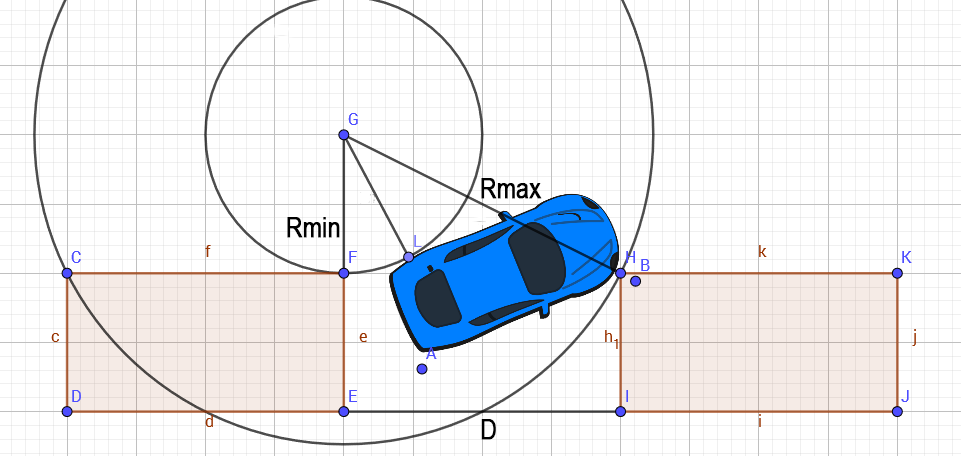
\includegraphics[scale=0.4]{vehicleParallelParkingAnalysis}
\caption[Analiza parkowania równoległego]{Analiza parkowania równoległego}
\end{figure}
	
\end{itemize}

Na powyższym rysunku zaznaczone zostały okręgi, minimalny i maksymalny, jakie zarysowuje pojazd podczas parkowania. Do obliczenia minimalnej długości miejsca parkingowego potrzebnej do wykonania parkowania w pojedynczym manewrze przyjmijmy następujące oznaczenia:
\begin{itemize}
\item $R_{min}$ – promień minimalnego okręgu wyznaczanego przez tylne koło znajdujące się po wewnętrznej stronie skrętu
\item $R_{max}$ – promień maksymalnego okręgu wyznaczanego przez przednie koło znajdujące się po zewnętrznej stronie skrętu
\item $d$ - minimalna długość miejsca parkingowego pozwalająca na parkowanie w pojedynczym manewrze:
\end{itemize}
$$
d = \sqrt{R^{2}_{max} - R^{2}_{min}}
$$

\subsection{Idea algorytmu}

Parametrami wejściowymi dla algorytmu wyznaczania ścieżki parkowania są następujące dane:
\begin{itemize}
	\item mapa,
	\item pojazd,
	\item wybrane miejsce parkingowe (zawiera ono dozwolony typ parkowania, tzn. równoległe lub prostopadłe).
\end{itemize}

Działanie samego algorytmu rozpoczyna się od sprawdzenia, która z opisanych w poprzednim podrozdziale sytuacji ma miejsce. Jeśli miejsce parkingowe jest zbyt małe to algorytm kończy działanie i zwraca informację, że zaparkowanie w danym miejscu nie było możliwe. Następnym krokiem jest sprawdzenie czy mamy do czynienia z parkowaniem równoległym, czy prostopadłym oraz czy naszym celem jest wyznaczenie ścieżki wjazdowej, czy wyjazdowej z miejsca parkingowego.

Zamiast jednak rozważać osobno w jaki sposób wygenerować ścieżkę parkowania umożliwiającą wjazd, a w jaki sposób ścieżkę umożliwiającą wyjazd z miejsca parkingowego wystarczy rozważyć tylko sytuację wyjazdu z danego miejsca. Takie podejście jest wystarczające, ponieważ mając wyznaczoną ścieżkę, umożliwiającą wyjazd z miejsca parkingowego możliwe jest uzyskanie ścieżki wjazdowej poprzez odwrócenie kolejności elementów wchodzących w skład tej ścieżki.

W przypadku parkowania prostopadłego wyznaczenie ścieżki parkowania jest zadaniem trywialnym i sprowadza się do ustawienia pojazdu idealnie na środku miejsca parkingowego, a następnie wycofywania pojazdu, aż do momentu, gdy cały znajdzie się na zewnątrz. Jeśli zadaniem algorytmu było wyznaczenie ścieżki wyjazdowej to jego działanie zostanie w tym momencie zakończone. W przypadku, gdy poszukiwana była ścieżka wjazdowa wystarczy odwrócić parametry wyznaczonej linii, po której ma poruszać się pojazd.  W obu przypadkach wyznaczona ścieżka składa się z pojedynczej linii.

Trudniejszym zadaniem jest wyznaczenie ścieżki parkowania równoległego. Na początek podobnie jak poprzednio należy ustawić pojazd na środku miejsca parkingowego. W następnym kroku pojazd jest wycofywany, aż do momentu, gdy jego tylna krawędź pokryje się z tylną krawędzią miejsca parkingowego (tutaj można rozważać sytuację idealną gdy tylna krawędź pojazdu zrównuje się z tylną krawędzią miejsca lub dać jakąś tolerancję, aby do tej krawędzi nie dojeżdżał i zachowywał określony odstęp). Gdy pojazd znajduje się już w takim ustawieniu rozpoczyna się główna pętla algorytmu, w której pojazd porusza się po kolejnych fragmentach okręgów do momentu, aż całkowicie znajdzie się poza miejscem parkingowym. 

Zanim przedstawiony zostanie opis kolejnych manewrów wykonywanych przez pojazd warto najpierw  obliczyć jaka ilość miejsca na takie manewry jest dostępna. Aby to zrobić wystarczy od długości miejsca parkingowego odjąć długość pojazdu. Wartość jaką otrzymamy to całkowita ilość dostępnego miejsca na wykonywanie kolejnych manewrów. Pojedynczy manewr na tym etapie algorytmu składa się z dwóch łuków, gładko połączonych, po przejechaniu których pojazd znajduje się w takiej samej orientacji jak przed wykonaniem manewru, ale przemieszcza się na koniec dostępnego miejsca oraz coraz bliżej wyjazdu z miejsca parkingowego.

Zakładając, że wyjazd z miejsca parkingowego znajduje się po lewej stronie pojazdu to pierwszy łuk będzie skierowany w lewo i będzie się kończył w połowie dostępnego miejsca. W tym punkcie koła pojazdu powinny zostać skręcone maksymalnie w drugą stronę, tak aby rozpoczął on ruch po drugim łuku i aby pojazd dojechał do końca dostępnego miejsca. W tym momencie pojazd powinien mieć taką samą orientację jak przed wykonaniem opisanych manewrów. Jeśli pojazd nie znajduje się jeszcze całkowicie poza miejscem parkingowym to ponownie wykonuje ruch po dwóch łukach, tym razem do tyłu. Operacje te są powtarzane do momentu całkowitego wyjazdu pojazdu z miejsca parkingowego.

\subsection{Pseudokod algorytmu parkowania równoległego}

W tym podrozdziale przedstawiony zostanie pseudokod opisanego powyżej algorytmu parkowania równoległego. Opis metody wyznaczania okręgów skrętu, które będą tu wykorzystane znajduje się w rozdziale ''Analiza ruchu pojazdu''.

\begin{pseudokod}
Algorytm parkowania
\begin{verbatim}
    jeżeli długość lub szerokość miejsca parkingowego jest mniejsza niż 
    długość lub szerokość pojazdu
        zwróć pustą ścieżkę parkingową
    ustaw pojazd na środku miejsca parkingowego w tej samej orientacji co miejsce
    cofnij pojazd do końca miejsca parkingowego

    liczba okręgów = 0
    kąt startowy = 0;
    kąt końcowy = 0;
	
    dopóki jakakolwiek część pojazdu znajduje się w miejscu parkingowym lub 
    liczba okręgów dodanych do ścieżki jest nieparzysta
    {
        wyznacz maksymalny kąt do którego pojazd może poruszać się po okręgu
        jeżeli liczba okręgów % 4 == 0
            okrąg = wyznacz lewy okrąg dla maksymalnego skrętu kół pojazdu 
                    i ruchu w przód dla którego kąt znajduje się w przedziale 
                    [kąt startowy, kąt końcowy]
        jeżeli liczba okręgów % 4 == 0
            okrąg = wyznacz prawy okrąg dla maksymalnego skrętu kół pojazdu 
                    i ruchu w przód dla którego kąt znajduje się w przedziale 
                    [2 * PI - kąt końcowy, 2 * PI + kąt startowy]
        jeżeli liczba okręgów % 4 == 0
            okrąg = wyznacz lewy okrąg dla maksymalnego skrętu kół pojazdu 
                    i ruchu w tył dla którego kąt znajduje się w przedziale 
                    [2 * PI + kąt startowy, 2 * PI - kąt końcowy]
        jeżeli liczba okręgów % 4 == 0
            okrąg = wyznacz prawy okrąg dla maksymalnego skrętu kół pojazdu 
                    i ruchu w tył dla którego kąt znajduje się w przedziale 
                    [kąt końcowy, kąt startowy]
        liczba okręgów++;
        dodaj okrąg do ścieżki parkowania
    }
    jeżeli ścieżka wyjazdowa
        odwróć ścieżkę parkowania	
    zwróć ścieżkę parkowania
\end{verbatim}
\end{pseudokod}

\subsection{Testy i dalszy rozwój algorytmu}

Testy algorytmu parkowania przebiegły pomyślnie i potwierdziły prawidłowe działanie algorytmu, zgodne z oczekiwaniami przy uprzednio przyjętych założeniach. Poniżej zaprezentowano przykładowe ścieżki parkowania, wygenerowane zarówno dla parkowania prostopadłego jak i równoległego.

\subsubsection{Parkowanie prostopadłe}

Przykładowe ścieżki parkowania:
\begin{itemize}
	\item wyznaczona ścieżka parkowania, gdy otoczenie miejsca parkingowego jest bezkolizyjne
	\begin{figure}[h!]
\centering
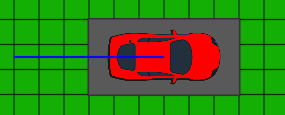
\includegraphics[scale=1.0]{parkingPathPerpendicular1}
\caption[Ścieżka parkowania prostopadłego]{Ścieżka parkowania prostopadłego}
\end{figure}
	\item sytuacja, w której algorytm zwraca informację, że zaparkowanie nie jest możliwe, choć w rzeczywistości taki manewr dałoby się wykonać (przeszkoda znajduje się zbyt blisko wyznaczonej ścieżki parkowania i powoduje kolizję z poruszającym się po tej ścieżce pojazdem).
	\begin{figure}[h!]
\centering
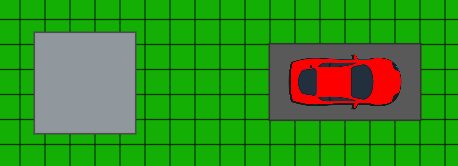
\includegraphics[scale=0.68]{parkingPathPerpendicular2}
\caption[Brak ścieżki umożliwiającej zaparkowanie prostopadłe]{Brak ścieżki umożliwiającej zaparkowanie prostopadłe}
\end{figure}
\end{itemize}

\subsubsection{Parkowanie równoległe}

Przykładowe ścieżki parkowania:
\begin{itemize}
	\item szerokie miejsce parkingowe – parkowanie w pojedynczym manewrze
	\begin{figure}[h!]
\centering
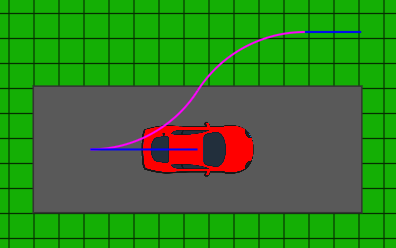
\includegraphics[scale=0.68]{parkingPathParallel1}
\caption[Parkowanie w szerokim miejscu parkingowym]{Parkowanie w szerokim miejscu parkingowym}
\end{figure}
	\item wąskie miejsce parkingowe – parkowanie w kilku manewrach
	\begin{figure}[h!]
\centering
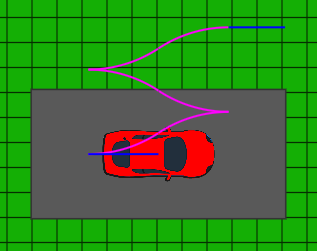
\includegraphics[scale=0.70]{parkingPathParallel2}
\caption[Parkowanie w wąskim miejscu parkingowym]{Parkowanie w wąskim miejscu parkingowym}
\end{figure}
	\item ekstremalnie wąskie miejsce parkingowe – parkowanie w bardzo dużej liczbie manewrów, ale wciąż możliwe
	\begin{figure}[h!]
\centering
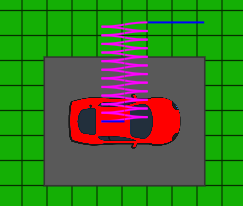
\includegraphics[scale=0.95]{parkingPathParallel3}
\caption[Parkowanie w ekstremalnie wąskim miejscu parkingowym]{Parkowanie w ekstremalnie wąskim miejscu parkingowym}
\end{figure}
\end{itemize}

Działanie algorytmu wyznaczania ścieżek parkingowych pokrywa wszystkie sytuacje jakie mogą wystąpić podczas wykonywania manewru parkowania, gdy otoczenie wokół miejsca parkingowego jest bezkolizyjne. Jednak w przypadku, gdy jakiś obiekt znajduje się zbyt blisko ścieżki parkowania i powoduje kolizję z poruszającym się po ścieżce pojazdem, to algorytm zwraca informację, że zaparkowanie w tym miejscu nie jest możliwe, choć w rzeczywistości, często dałoby się taką przeszkodę ominąć i zakończyć manewr parkowania pomyślnie.  Dalszym krokiem w rozwoju algorytmu byłoby więc wykrywanie takich sytuacji i próba omijania przeszkód, aby możliwe było pomyślne dokończenie manewru, a nie natychmiastowe kończenie działania algorytmu. Nie ma natomiast żadnych zastrzeżeń co do czasu działania algorytmu. Wszystkie obliczenia wykonywane są błyskawicznie i odpowiedź algorytmu jest niemal natychmiastowa.

\chapter{Instrukcja użytkownika}

Interfejs aplikacji został podzielony na 6 zakładek, w których kolejno znajduje się ekran startowy, edytor map, edytor pojazdów, planer ruchu, moduł wizualizacji oraz zakładka umożliwiająca zmianę ustawień aplikacji. Funkcjonalności i obsługa każdej z zakładek została przedstawiona w poniższych podrozdziałach.

\section{Ekran startowy}

Zrzut ekranu startowego przedstawiono na poniższym obrazku.

\begin{figure}[h!]
\centering
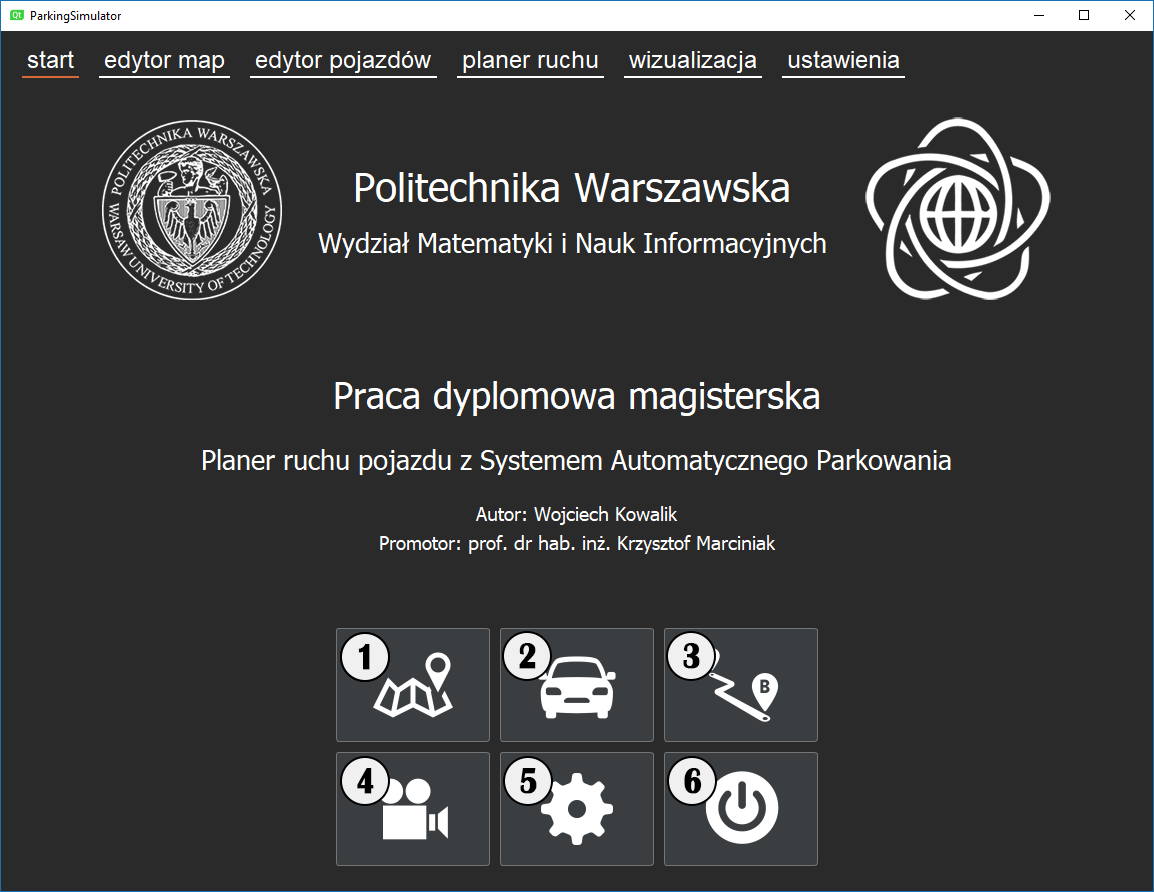
\includegraphics[scale=0.5]{instructionStart}
\caption[Ekran startowy - zrzut ekranu]{Ekran startowy - zrzut ekranu}
\end{figure}

Ekran ten zawiera następujące przyciski, które umożliwiają szybkie przejście do poszczególnych modułów aplikacji:
\begin{itemize}
	\item \textbf{[1]} - umożliwia przejście do edytora map,
	\item \textbf{[2]} - umożliwia przejście do edytora pojazdów,
	\item \textbf{[3]} - umożliwia przejście do planera ruchu pojazdu,
	\item \textbf{[4]} - umożliwia przejście do modułu wizualizacji,
	\item \textbf{[5]} - umożliwia przejście do ustawień aplikacji,
	\item \textbf{[6]} - umożliwia zamknięcie aplikacji.
\end{itemize}

\section{Edytor map}

Zrzut ekranu przedstawiający widok edytora map przedstawiono na poniższym obrazku.

\begin{figure}[h!]
\centering
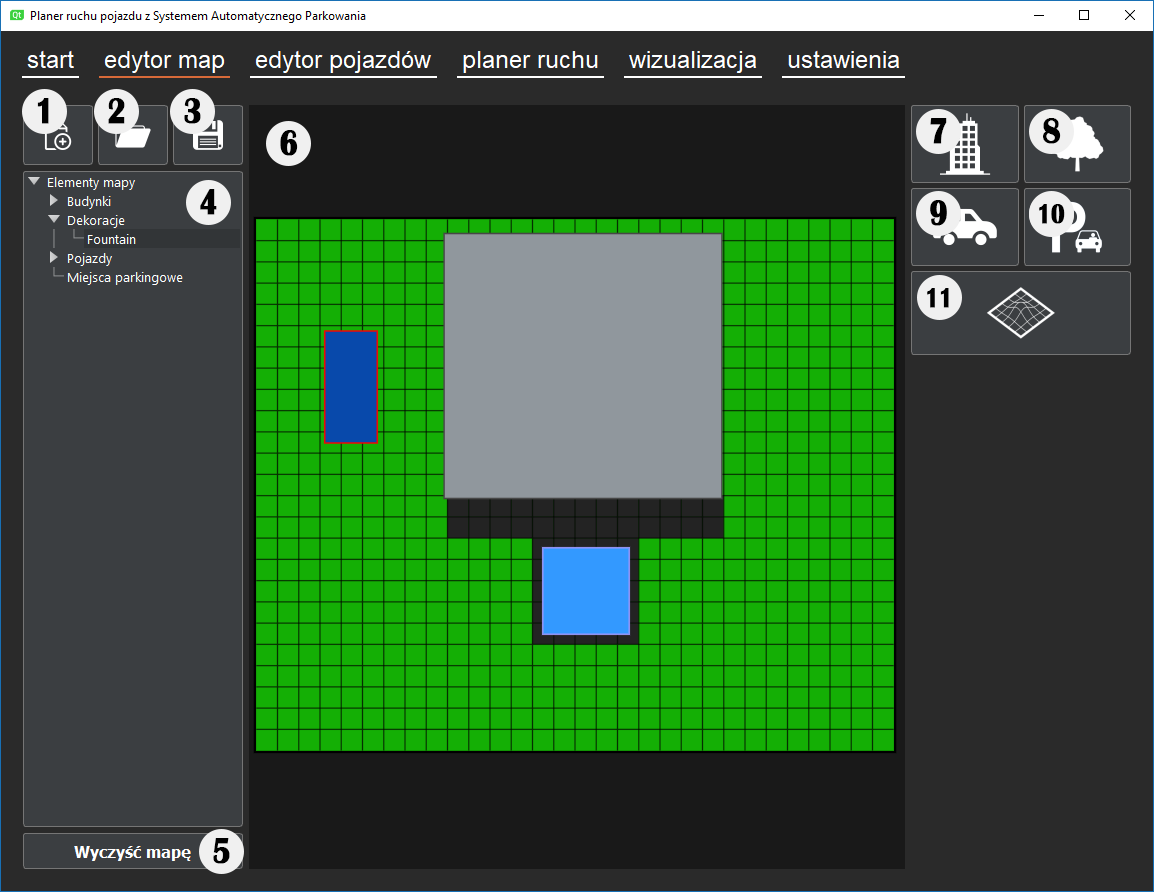
\includegraphics[scale=0.5]{instructionMapEditor}
\caption[Edytor map - zrzut ekranu]{Edytor map - zrzut ekranu}
\end{figure}

Edytor map zawiera następujące okna i przycisku:
\begin{itemize}
	\item \textbf{[1]} - przycisk umożliwiający stworzenie nowej mapy,
	\item \textbf{[2]} - przycisk umożliwiający otwarcie mapy zapisanej do pliku,
	\item \textbf{[3]} - przycisk umożliwiający zapisanie mapy do pliku,
	\item \textbf{[4]} - drzewo zawierające obiekty dodane do mapy,
	\item \textbf{[5]} - przycisk umożliwiający natychmiastowe usunięcie wszystkich obiektów znajdujących się na mapie,
	\item \textbf{[6]} - interaktywny edytor mapy,
	\item \textbf{[7]} - przycisk umożliwiający dodanie obiektu będącego budynkiem do mapy,
	\item \textbf{[8]} - przycisk umożliwiający dodanie dekoracyjnego obiektu do mapy,
	\item \textbf{[9]} - przycisk umożliwiający dodanie pojazdu do mapy,
	\item \textbf{[10]} - przycisk umożliwiający dodanie miejsca parkingowego do mapy,
	\item \textbf{[11]} - przycisk umożliwiający zmianę rodzaju terenu na mapie.
\end{itemize}

Aby utworzyć nową mapę użytkownik powinien nacisnąć przycisk \textbf{[1]}, a następnie, w nowo otwartym oknie podać wymiary mapy i zatwierdzić operację. Po kliknięciu na przycisk \textit{''Utwórz''} nowa mapa zostanie stworzona i zastąpi mapę aktualnie znajdującą się w edytorze map.

\begin{figure}[h!]
\centering
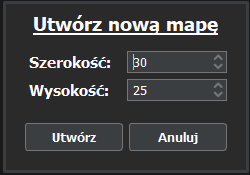
\includegraphics[scale=1.0]{instructionCreateMap}
\caption[Okno tworzenia nowej mapy]{Okno tworzenia nowej mapy}
\end{figure}

Po kliknięciu na jeden z przycisków umożliwiających dodanie nowego obiektu do mapy, zostanie wyświetlone okno dialogowe podobne do tego przedstawionego na poniższym zrzucie ekranu. Użytkownik ma możliwość wyboru konkretnego modelu danego obiektu jaki chce dodać do mapy, wpisania jego nazwy oraz podania wymiarów. Nie zaleca się jednak zmiany wymiarów obiektów posiadających skomplikowany model, gdyż jeśli podczas zmiany nie zostaną zachowane odpowiednie proporcje poszczególnych wymiarów, to obiekt może zostać znacząco zdeformowany.

\begin{figure}[h!]
\centering
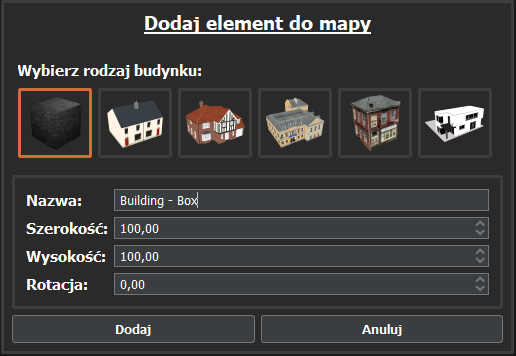
\includegraphics[scale=0.9]{instructionAddMapElement}
\caption[Okno dodawania nowego elementu do mapy]{Okno dodawania nowego elementu do mapy}
\end{figure}

Po wybraniu odpowiedniego modelu i zatwierdzeniu całej operacji poprzez kliknięcie na przycisk ''Dodaj'' należy umieścić nowo dodany obiekt w odpowiednim miejscu na mapie. Podczas poruszania obiektem po mapie może on zmieniać kolor z zielonego na czerwony (lub inne kolory wybrane w ustawieniach aplikacji). Kolor obiektu symbolizuje to czy obiekt można umieścić w danym miejscu czy nie. Aby umieszczenie obiektu było możliwe musi on w całości znajdować się w obszarze mapy i nie może kolidować z innymi obiektami znajdującymi  się na mapie.

Obiekty dodane do mapy można poddawać ponownej edycji. Aby to zrobić należy kliknąć w obiekt na mapie lub wybrać interesujący nas element z drzewa obiektów. Obiekt może być poddany operacji translacji, rotacji i skalowania. Po zaznaczeniu dowolnego obiektu, pod przyciskami służącymi dodawaniu nowych elementów do mapy wyświetlona zostanie sekcja wyświetlająca właściwości danego obiektu. Dowolny obiekt może zostać również usunięty z mapy.

Podczas korzystania z edytora map jak i kolejnych modułów, które posiadają obszar interaktywny w trybie 2D, możliwe jest przybliżanie określonych fragmentów mapy używając w tym celu kółka myszki, a także przesuwanie mapy. Aby przesunąć mapę należy nacisnąć środkowy przycisk myszki i poruszyć myszką w odpowiednią stronę.

\section{Edytor pojazdów}

Edytor pojazdów umożliwia stworzenie nowego pojazdu. Pozwala on na ustawienie przez użytkownika takich parametrów pojazdu jak:
\begin{itemize}
	\item nazwa,
	\item długość i szerokość,
	\item rozstaw osi oraz rozstaw kół,
	\item maksymalny kąt skrętu przednich kół.
\end{itemize}

Ekran edytora pojazdu został przedstawiony na poniższym zrzucie ekranu.

\begin{figure}[h!]
\centering
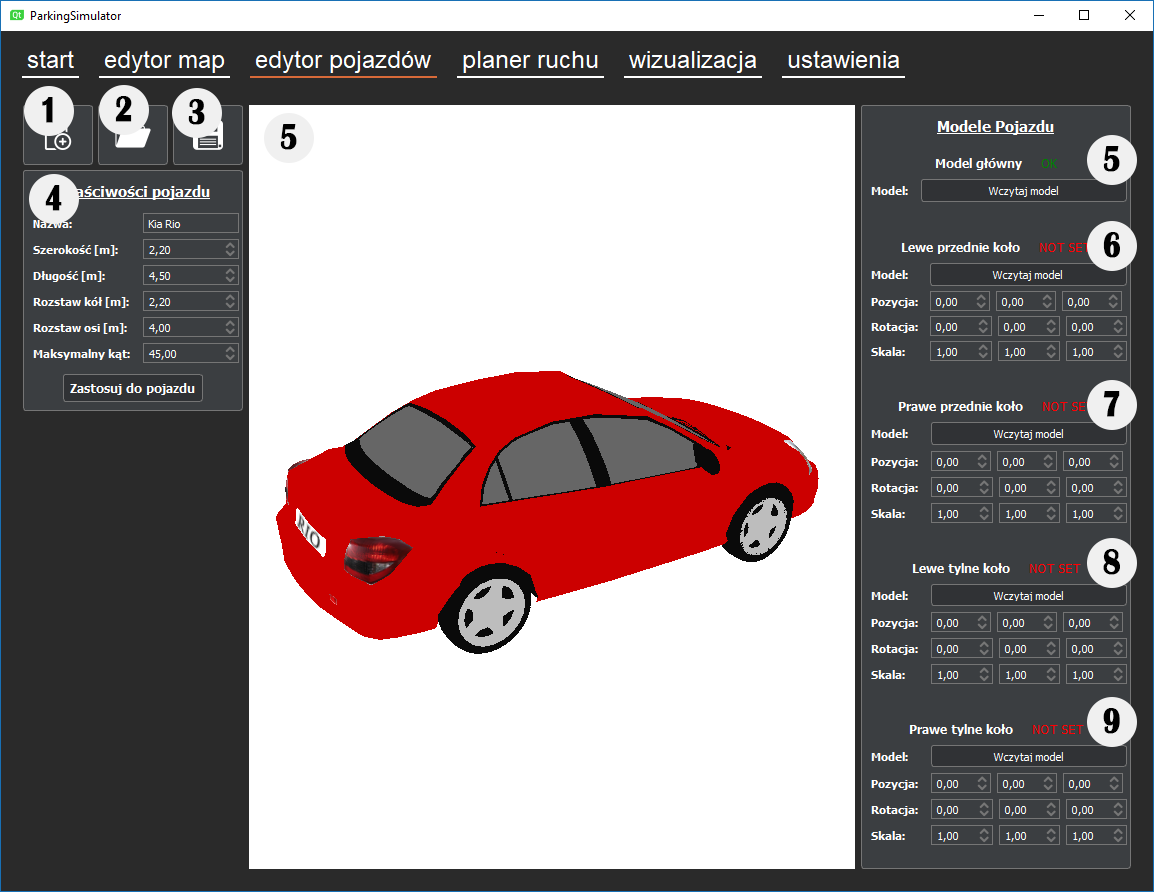
\includegraphics[scale=0.5]{instructionVehicleEditor}
\caption[Edytor pojazdów - zrzut ekranu]{Edytor pojazdów - zrzut ekranu}
\end{figure}

Na ekranie edytora pojazdów znajdują się następujące przyciski i sekcje:
\begin{itemize}
	\item \textbf{[1]} - przycisk pozwalający na utworzenie nowego pojazdu
	\item \textbf{[2]} - przycisk pozwalający na wczytanie pojazdu z pliku,
	\item \textbf{[3]} - przycisk pozwalający na zapis pojazdu do pliku,
	\item \textbf{[4]} - sekcja umożliwiająca konfigurację różnych parametrów pojazdu,
	\item \textbf{[5]} - okno z podglądem pojazdu 3D,
	\item \textbf{[6]} - sekcja umożliwiająca dodanie głównego modelu pojazdu,
	\item \textbf{[7]}, \textbf{[8]}, \textbf{[9]}, \textbf{[10]} - sekcje umożliwiające dodanie kolejny modeli wszystkich kół pojazdu oraz ich odpowiednie transformacje w celu dopasowania i poprawnego ustawienia względem głównego modelu.
\end{itemize}

Aby utworzyć nowy pojazd należy kliknąć w przycisk ''Utwórz nowy pojazd'', a następnie wczytać główny model pojazdu oraz ustawić parametry pojazdu. Dodanie modeli poszczególnych kół jest opcjonalne, jednak model główny musi być dodany obowiązkowo.

Edytor pojazdów jest edytorem 3D. Aby poruszać kamerą w tym edytorze należy użyć myszki do wykonywania obrotów, natomiast do przesuwania kamery służą przyciski WSAD.

\section{Planer ruchu}

Zrzut ekranu planera ruchu przedstawiono na poniższym obrazku.

\begin{figure}[h!]
\centering
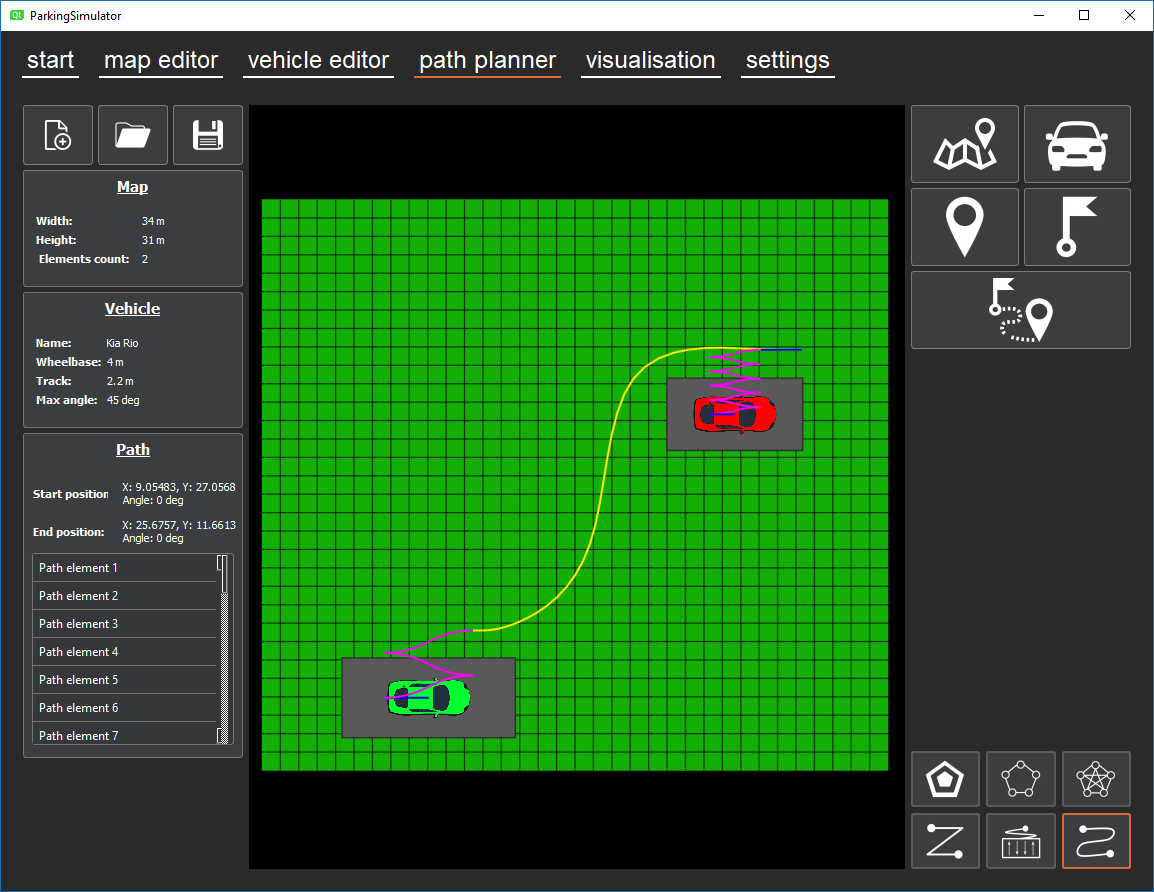
\includegraphics[scale=0.5]{instructionPathPlanner}
\caption[Planer ruchu - zrzut ekranu]{Planer ruchu - zrzut ekranu}
\end{figure}

Na ekranie tym znajdują się następujące przyciski i sekcje:
\begin{itemize}
	\item \textbf{[1]} - przycisk umożliwiający utworzenie nowej symulacji,
	\item \textbf{[2]} - przycisk umożliwiający wczytanie symulacji z pliku,
	\item \textbf{[3]} - przycisk umożliwiający zapis symulacji do pliku,
	\item \textbf{[4]} - sekcja prezentująca informacje o wczytanej mapie,
	\item \textbf{[5]} - sekcja prezentująca informacje o wczytanym pojeździe,
	\item \textbf{[6]} - sekcja prezentująca informacje na temat wygenerowanej ścieżki,
	\item \textbf{[7]} - okno prezentujące mapę oraz inne elementy, których widok może zostać włączony/wyłączony,
	\item \textbf{[8]} - przycisk umożliwiający dodanie mapy do symulacji,
	\item \textbf{[9]} - przycisk umożliwiający wybranie pojazdu,
	\item \textbf{[10]} - przycisk umożliwiający ustawienie położenia początkowego,
	\item \textbf{[11]} - przycisk umożliwiający ustawienie położenia końcowego,
	\item \textbf{[12]} - przycisk umożliwiający rozpoczęcie procesu wyznaczania trajektorii dla pojazdu,
	\item \textbf{[13]} - przycisk umożliwiający włączenie/wyłączenie widoku powiększonych przeszkód na mapie,
	\item \textbf{[14]} - przycisk umożliwiający włączenie/wyłączenie widoku grafu Voronoi,
	\item \textbf{[15]} - przycisk umożliwiający włączenie/wyłączenie widoku zmodyfikowanego grafu Voronoi, na którym prowadzone są obliczenia,
	\item \textbf{[16]} - przycisk umożliwiający włączenie/wyłączenie widoku ścieżki wyznaczonej w grafie (łamanej),
	\item \textbf{[17]} - przycisk umożliwiający włączenie/wyłączenie widoku wyznaczonych ścieżek parkingowych,
	\item \textbf{[18]} - przycisk umożliwiający włączenie/wyłączenie widoku finalnej ścieżki.
\end{itemize}

Aby rozpocząć planowanie ruchu pojazdu należy utworzyć nową symulację oraz dodać do niej mapę i pojazd. Następnie użytkownik musi ustawić położenie początkowe oraz końcowe pojazdu. Po ustawieniu każdego z wymienionych parametrów informacje o nim wyświetlane są w jednej z sekcji znajdujących się po lewej stronie okna. Następnie należy kliknąć na przycisk ''Wyznacz ścieżkę''. Otwarte zostanie następujące okno:

\newpage

\begin{figure}[h!]
\centering
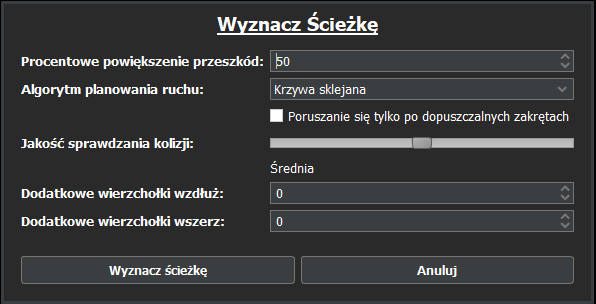
\includegraphics[scale=1.0]{instructionFindPath}
\caption[Okno z parametrami do wyznaczania ścieżki]{Okno z parametrami do wyznaczania ścieżki}
\end{figure}

W nowo otwartym oknie użytkownik ma możliwość ustawienia procentowej wartości szerokości pojazdu o jaką zostaną powiększone wszystkie przeszkody znajdujące się na mapie. Następnie zachodzi konieczność wyboru algorytmu planowania ruchu oraz w przypadku wybrania algorytmu wpisywania łuków użytkownik musi określić, czy zgadza się tylko na skręty dopuszczalne dla danego pojazdu, czy na dowolne. Kolejnym parametrem jest jakość wykrywania kolizji. Zaleca się pozostawienie jej na poziomie średnim, gdyż zbyt niska wartość tego parametru może spowodować, że zaczną pojawiać się kolizje pojazdu z innymi obiektami na mapie podczas przejazdu wyznaczoną trajektorią, natomiast zbyt wysoka wartość spowoduje znaczące wydłużenie czasu obliczeń. Pozostałe dwa parametry służą do określenia przez użytkownika gęstości siatki sztucznych wierzchołków, które zostaną dodane do konstruowanego grafu.

Po ustawieniu powyższych parametrów należy kliknąć w przycisk ''Znajdź ścieżkę'' i proces planowania ruchu pojazdu się rozpocznie. Podczas trwania obliczeń wszystkie przyciski planera ruchu zostaną zablokowane, jednak użytkownik będzie miał możliwoość przerwania obliczeń w dowolnym momencie. Po zakończeniu obliczeń zostanie wyświetlony komunikat informujący o powodzeniu bądź niepowodzeniu procesu planowania.

\section{Wizualizacja}

Zrzut ekranu przedstawiający moduł wizualizacji przedstawiono na poniższym obrazku.

\begin{figure}[h!]
\centering
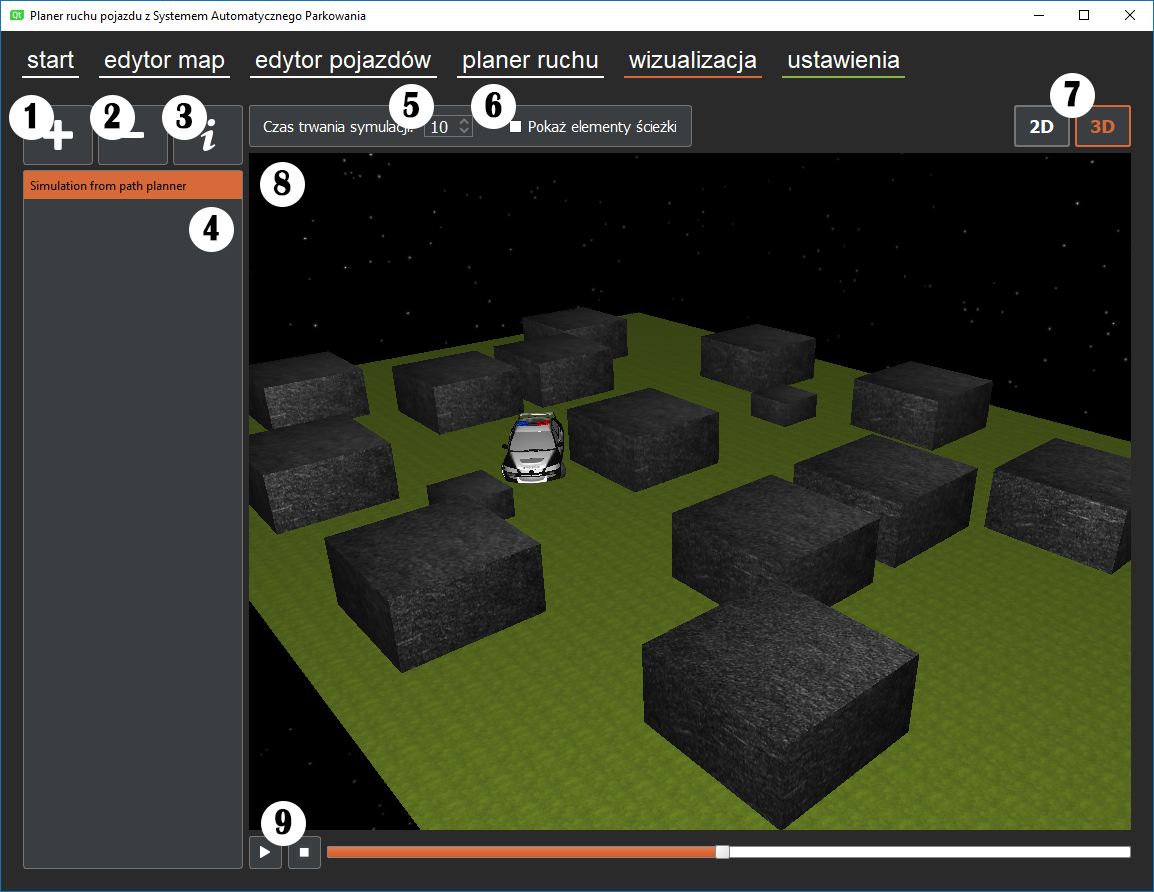
\includegraphics[scale=0.5]{instructionVisualisation}
\caption[Wizualizacja - zrzut ekranu]{Wizualizacja - zrzut ekranu}
\end{figure}

Ekran modułu wizualizacji zawiera następujące przyciski i sekcje:
\begin{itemize}
	\item \textbf{[1]} - przycisk umożliwiający dodanie nowej symulacji,
	\item \textbf{[2]} - przycisk umożliwiający usunięcie wybranej symulacji,
	\item \textbf{[3]} - przycisk umożliwiający wyświetlenie szczegółowych informacji na temat wybranej symulacji,
	\item \textbf{[4]} - lista zawierająca dodane symulacje,
	\item \textbf{[5]} - spin box umożliwiający ustawienie czasu trwania przejazdu,
	\item \textbf{[6]} - checkbox umożliwiający włączenie/wyłączenie widoku wyznaczonej ścieżki,
	\item \textbf{[7]} - przyciski umożliwiające zmianę widoku pomiędzy 2D, a 3D,
	\item \textbf{[8]} - okno wizualizacji,
	\item \textbf{[9]} - panel sterowania wizualizacją - umożliwia rozpoczęcie odtwarzania, pauzowanie i przewijanie do dowolnego momentu symulacji.
\end{itemize}

W module wizualizacji użytkownik ma możliwość dodania nowej symulacji do wyświetlenia poprzez kliknięcie na przycisk ''Dodaj symulację''. Ma również możliwość usunięcia dodanej już symulacji, bądź wyświetlenia szczegółowych informacji na je temat. Po dodaniu symulacji aktywowana jest możliwość wizualizacji przejazdu pomiędzy położeniem początkowym i końcowym. Wizualizacja może odbywać się zarówno w trybie 2D jak i 3D. W trybie 3D użytkownik może obracać kamerę przy użyciu myszki, natomiast przesuwanie kamery realizowane jest poprzez klawisze WSAD. Ponadto użytkownik ma możliwość ustawienia czasu trwania przejazdu oraz włączenia/wyłączenia widoku wyznaczonej trajektorii w trybie 2D.

Po wybraniu jednej z dodanych symulacji i kliknięciu na przycisk ''Informacje o symulacji'' wyświetlone zostanie okno przedstawione na poniższym zrzucie ekranu. Zawiera ono wszystkie podstawowe informacje na temat wybranej przez użytkownika symulacji, takie jak np. ilość elementów wchodzących w skład ścieżki, czy długość wyznaczonej trajektorii.

\begin{figure}[h!]
\centering
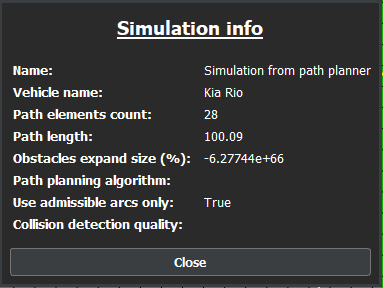
\includegraphics[scale=1.0]{instructionSimulationInfo}
\caption[Okno z informacjami o bieżącej symulacji]{Okno z informacjami o bieżącej symulacji}
\end{figure}

\section{Ustawienia}

Zakładka ''Ustawienia'' umożliwia zmianę podstawowych ustawień aplikacji. Możliwa jest zmiana języka, poprzez wybranie interesującego języka z rozwijanej listy. Możliwa jest również zmiana wyglądu wielu elementów wyświetlanych na mapie. Zmiany szerokości tych elementów użytkownik dokonuje za pomocą odpowiedniego spinboxa, odpowiadającego danemu elementowi. Aby dokonać zmiany koloru danego elementu należy kliknąć w kolor przy elemencie który chcemy zmienić. Zostanie wyświetlone okienko dialogowe, które umożliwi wybór nowego koloru. Po zatwierdzeniu wyboru kolor zostanie zmieniony. Aby jednak jakiekolwiek zmiany weszły w życie przed opuszczeniem zakładki ''Ustawienia'' użytkownik musi zapisać zmiany których dokonał, poprzez kliknięcie w przycisk ''Zapisz zmiany''. 

Poniżej zrzut ekranu prezentujący widok zakładki.

\begin{figure}[h!]
\centering
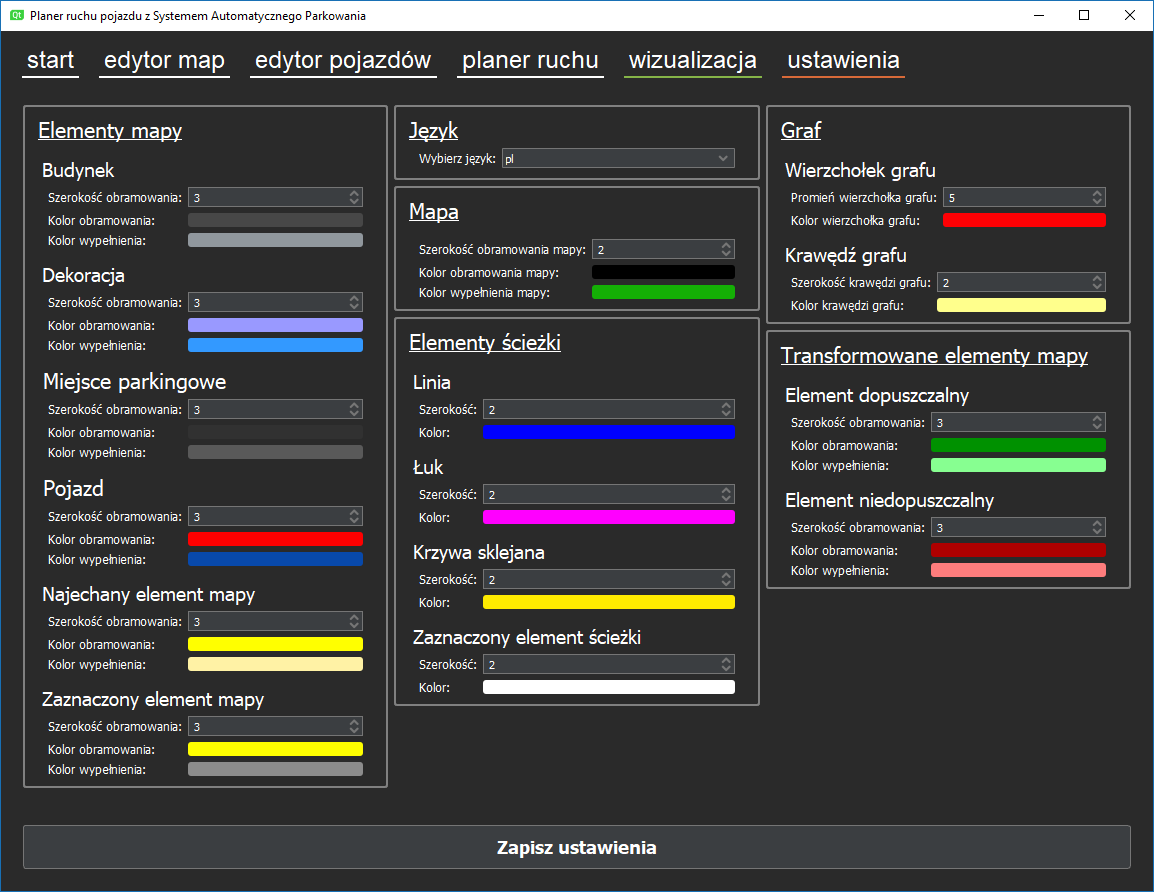
\includegraphics[scale=0.5]{instructionSettings}
\caption[Ustawienia - zrzut ekranu]{Ustawienia - zrzut ekranu}
\end{figure}

\chapter{Zakończenie}

Opracowanie planera ruchu pojazdu wraz z systemem automatycznego parkowania pozwoliło na praktyczne wykorzystanie wiadomości zdobytych na studiach drugiego stopnia, specjalność ''\textit{Projektowanie systemów CAD/CAM}''. Aplikacja została przygotowana w taki sposób, aby możliwie jak najbardziej odwzorowywać sytuacje, które występują w rzeczywistym świecie. 

Tym co odróżnia jednak zaprojektowany system od rzeczywistych autopilotów i modułów parkowania parkowania jest fakt, iż w opracowanej aplikacji wszystkie dane są dostępne od początku jego działania, tzn. planer ma wiedzę na temat wszystkich miejsc parkingowych, a asystent parkowania zna wszelkie parametry miejsca, w którym pojazd chce zaparkować. W rzeczywistym świecie informacje te nie są dostępne od początku i pojazd gromadzi je na bieżąco podczas ruchu, za pomocą wielu różnych czujników umieszczonych z każdej strony pojazdu. Ponadto otoczenie pojazdu w zaimplementowanej aplikacji jest statyczne - żadne obiekty na mapie poza pojazdem nie mogą się poruszać. W rzeczywistości taka idealna sytuacje nie występuje nigdy i wszystkie systemy muszą na bieżąco adaptować się do zmieniającego się otoczenia.

Niemniej jednak opracowana aplikacja z powodzeniem wykorzystuje niektóre pomysły, które używane są również w komercyjnych rozwiązaniach, a jej działanie pozwala przynajmniej w przybliżony sposób zobaczyć w jak działają rzeczywiste systemy planowania ruchu i moduły automatycznego parkowania.

% -------------------- 6. Bibliografia -----------------------
% Bibliografia leksykograficznie wg nazwisk autorów

\begin{thebibliography}{20}%jak ktoś ma więcej książek, to niech wpisze większą liczbę
% \bibitem[numerek]{referencja} Autor, \emph{Tytuł}, Wydawnictwo, rok, strony
% cytowanie: \cite{referencja1, referencja 2,...}

\bibitem[1]{Ktos} Sungwoo CHOI, Clément Boussard, Brigitte d’Andréa-Novel, \emph{Easy Path Planning and Robust Control for Automatic Parallel Parking}, 2011.
\bibitem[2]{Innyktos}  Jian-Min Wang, Sen-Tung Wu, Chao-Wei Ke, Bo-Kai Tzeng, \emph{Parking Path Programming Strategy for Automatic Parking System}, 2013.
\bibitem[3]{B} prof. dr hab. inż Krzysztof Marciniak, \emph{Wykłady z Programowania Urządzeń Sterowanych Numerycznie oraz Modelowania Geometrycznego}, Politechnika Warszawska, Wydział Matematyki i Nauk Informacyjnych, 2017.
\bibitem[4]{H} \emph{Ackermann Steering Geometry}, $https://en.wikipedia.org/wiki/AckermannSteeringGeometry$
\bibitem[5]{A} Tomasz Niechaj, \emph{Asystent parkowania}, $http://antyweb.pl/asystent-parkowania-jak-to-dziala-czy-rzeczywiscie-wyrecza-kierowce$
\end{thebibliography}
\thispagestyle{empty}


% --- 7. Wykaz symboli i skrótów - jeśli nie ma, zakomentować
%\chapter*{Wykaz symboli i skrótów}

%\begin{tabular}{cl}
%nzw. & nadzwyczajny \\
%* & operator gwiazdka \\
%$\widetilde{}$ & tylda
%\end{tabular}
%\thispagestyle{empty}


% ----- 8. Spis rysunków - jeśli nie ma, zakomentować --------
\listoffigures
\thispagestyle{empty}


% ------------ 9. Spis tabel - jak wyżej ------------------
\renewcommand{\listtablename}{Spis tabel}
\listoftables
\thispagestyle{empty}



% 10. Spis załączników - jak nie ma załączników, to zakomentować lub usunąć

%\chapter*{Spis załączników}
%\begin{enumerate}[itemsep = 0pt]
%\item Załącznik 1
%\item Załącznik 2
%\end{enumerate}
%\thispagestyle{empty}

% --------------------- 11. Załączniki ---------------------
% to jest po to, żeby było wiadomo, że załączniki znajdują się na końcu pracy

%\newpage
%\pagestyle{empty} 
%Załącznik 1, załącznik 2

\end{document}
